\chapter{Case Study: a 1/2-spin XYZ Heisenberg Chain Coupled to Two External Baths}
\label{Chapter3}

\section{The Model}
We are going to consider a Heisenberg XYZ chain of N $\frac{1}{2}$-spin, coupled to two external reservoirs positioned at the boundaries of the chain. The density matrix describing the chain evolves according to the Lindblad master equation
\begin{equation}
    \frac{d\rho}{dt} = -i[H, \rho] - \sum_{a=1}^{2}\gamma_a\Bigl(\frac{1}{2}L_a^{\dagger}L_a\rho + \frac{1}{2}\rho L_a^{\dagger}L_a - L_a\rho L_a^{\dagger}\Bigl),
\end{equation}
$H$ being the Hamiltonian of the model:
\begin{equation}
\label{ham_chain}
    H = \sum_{i = 1}^{N-1} (J_x \sigma_i^x \sigma_{i+1}^x + J_y \sigma_i^y \sigma_{i+1}^y + J_z \sigma_i^z \sigma_{i+1}^z),
\end{equation}
and the $\gamma_a$ being bath-coupling strength parameters. The $L_a$ are the Lindblad operators representing the single-spin bath coupled to the first and the last spin of the chain:
\begin{equation}
    L_1 = \frac{1}{2}(\sigma_x + i\sigma_y), \quad L_2 = \frac{1}{2}(\sigma_x - i\sigma_y).
\end{equation}

As disclosed previously, we are going to study this physical system through three numerical method: the QT method, the CSR method and the MPO method. We will see how everyone of these methods will be useful until they reach their own limits; examining these limits will be interesting and advantageous to set a benchmark [for numerical methods].

In the following sections, we will study three fundamental observables for the analysis of a XYZ Heisenberg chain: the magnetization profile, the two-point correlation function, the spin current; in particular, we will examine them in chains of different lengths: 4, 8, 12, 16, 32 sites. 

Before we begin the analysis, a look to the convergence of the three methods for every chain length is worthwhile. In this way, we will be able to set the method parameters in order to obtain  plausible results.

\section{Convergence}

\begin{figure}[H]
    \label{fig:convergence_mpo_8sites}
    \centering
    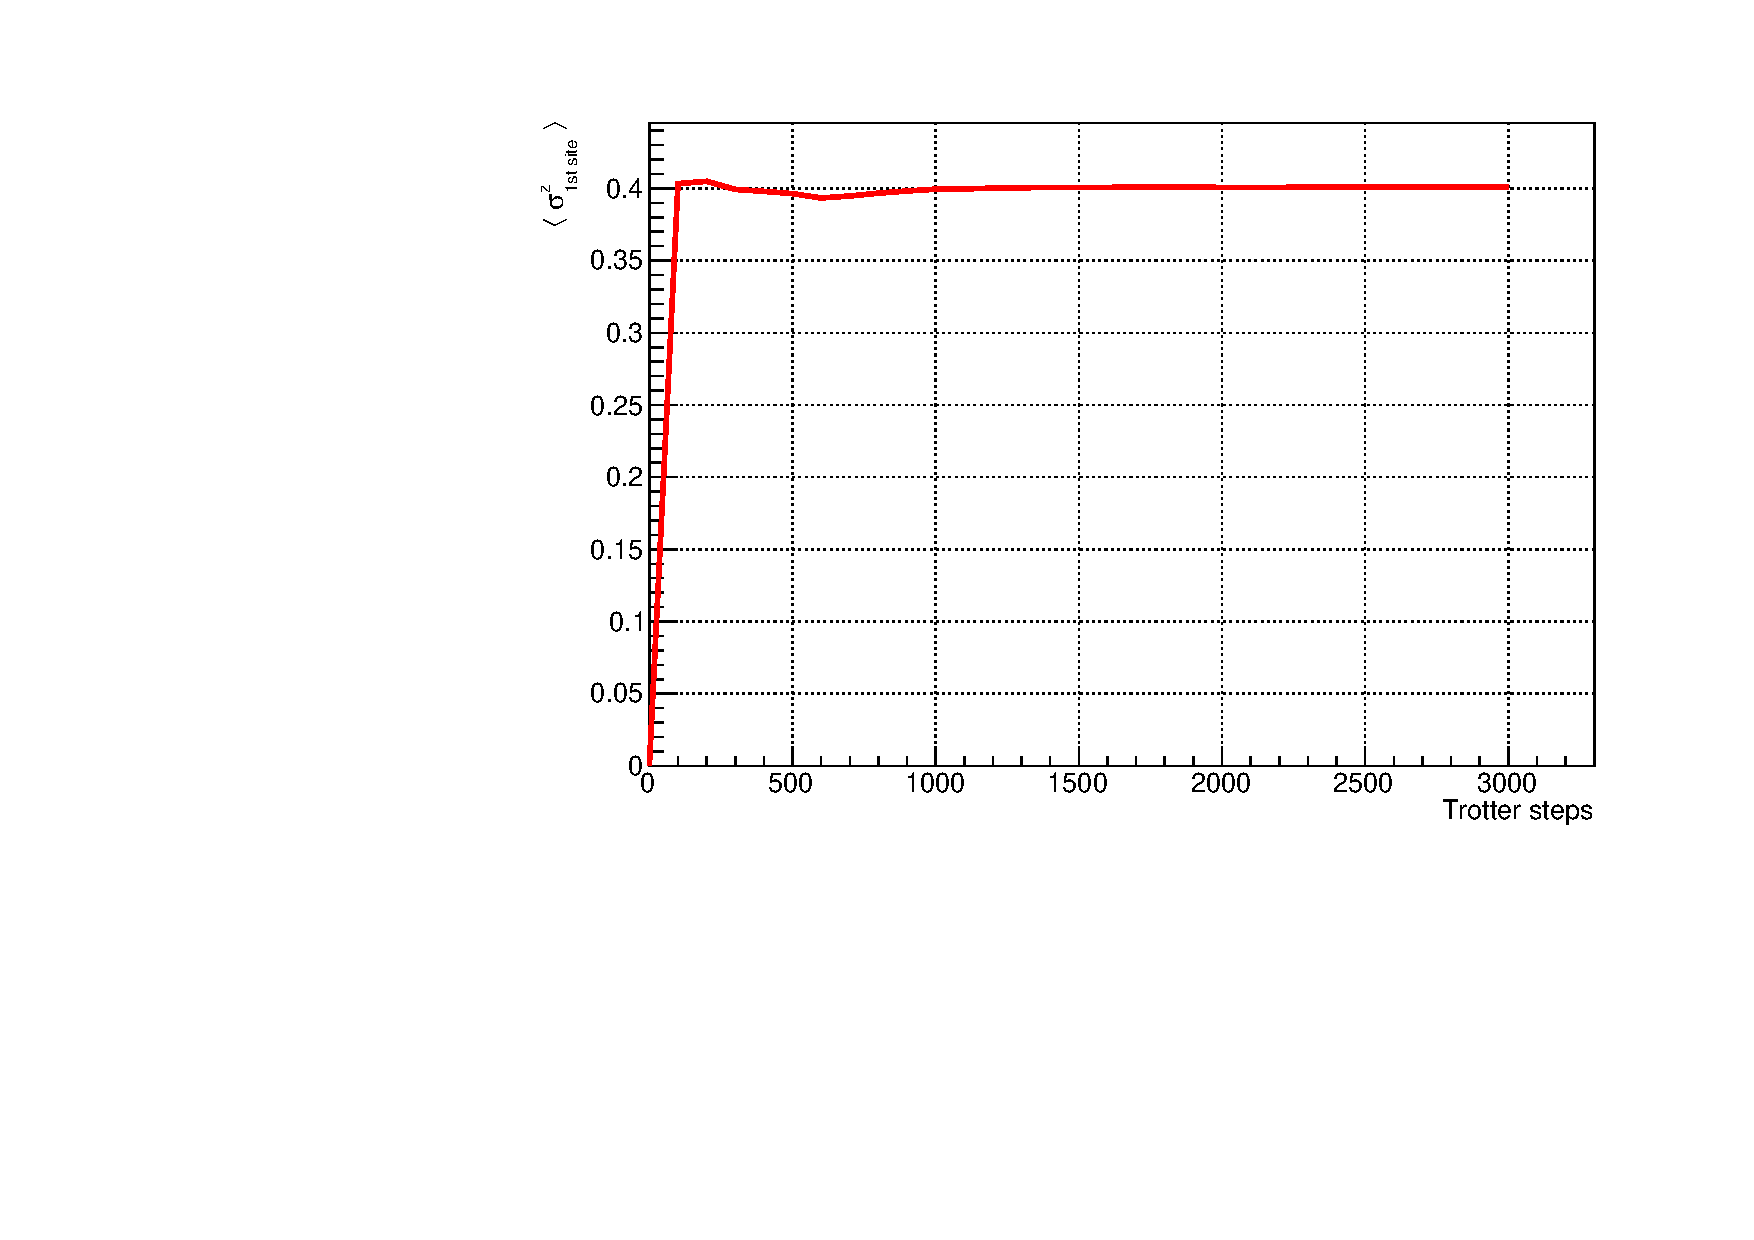
\includegraphics[scale=0.7]{Figures/convergence/Convergence_s8T3000J1051.pdf}
    \caption{Study of convergence of the MPO method for a 8-sites chain, for bond dimension m = 100 and T = 3000.}
    \label{fig:convergenceMPO_8sites}
\end{figure}

\begin{figure}[H]
    \label{fig:convergence_mpo_8sites}
    \centering
    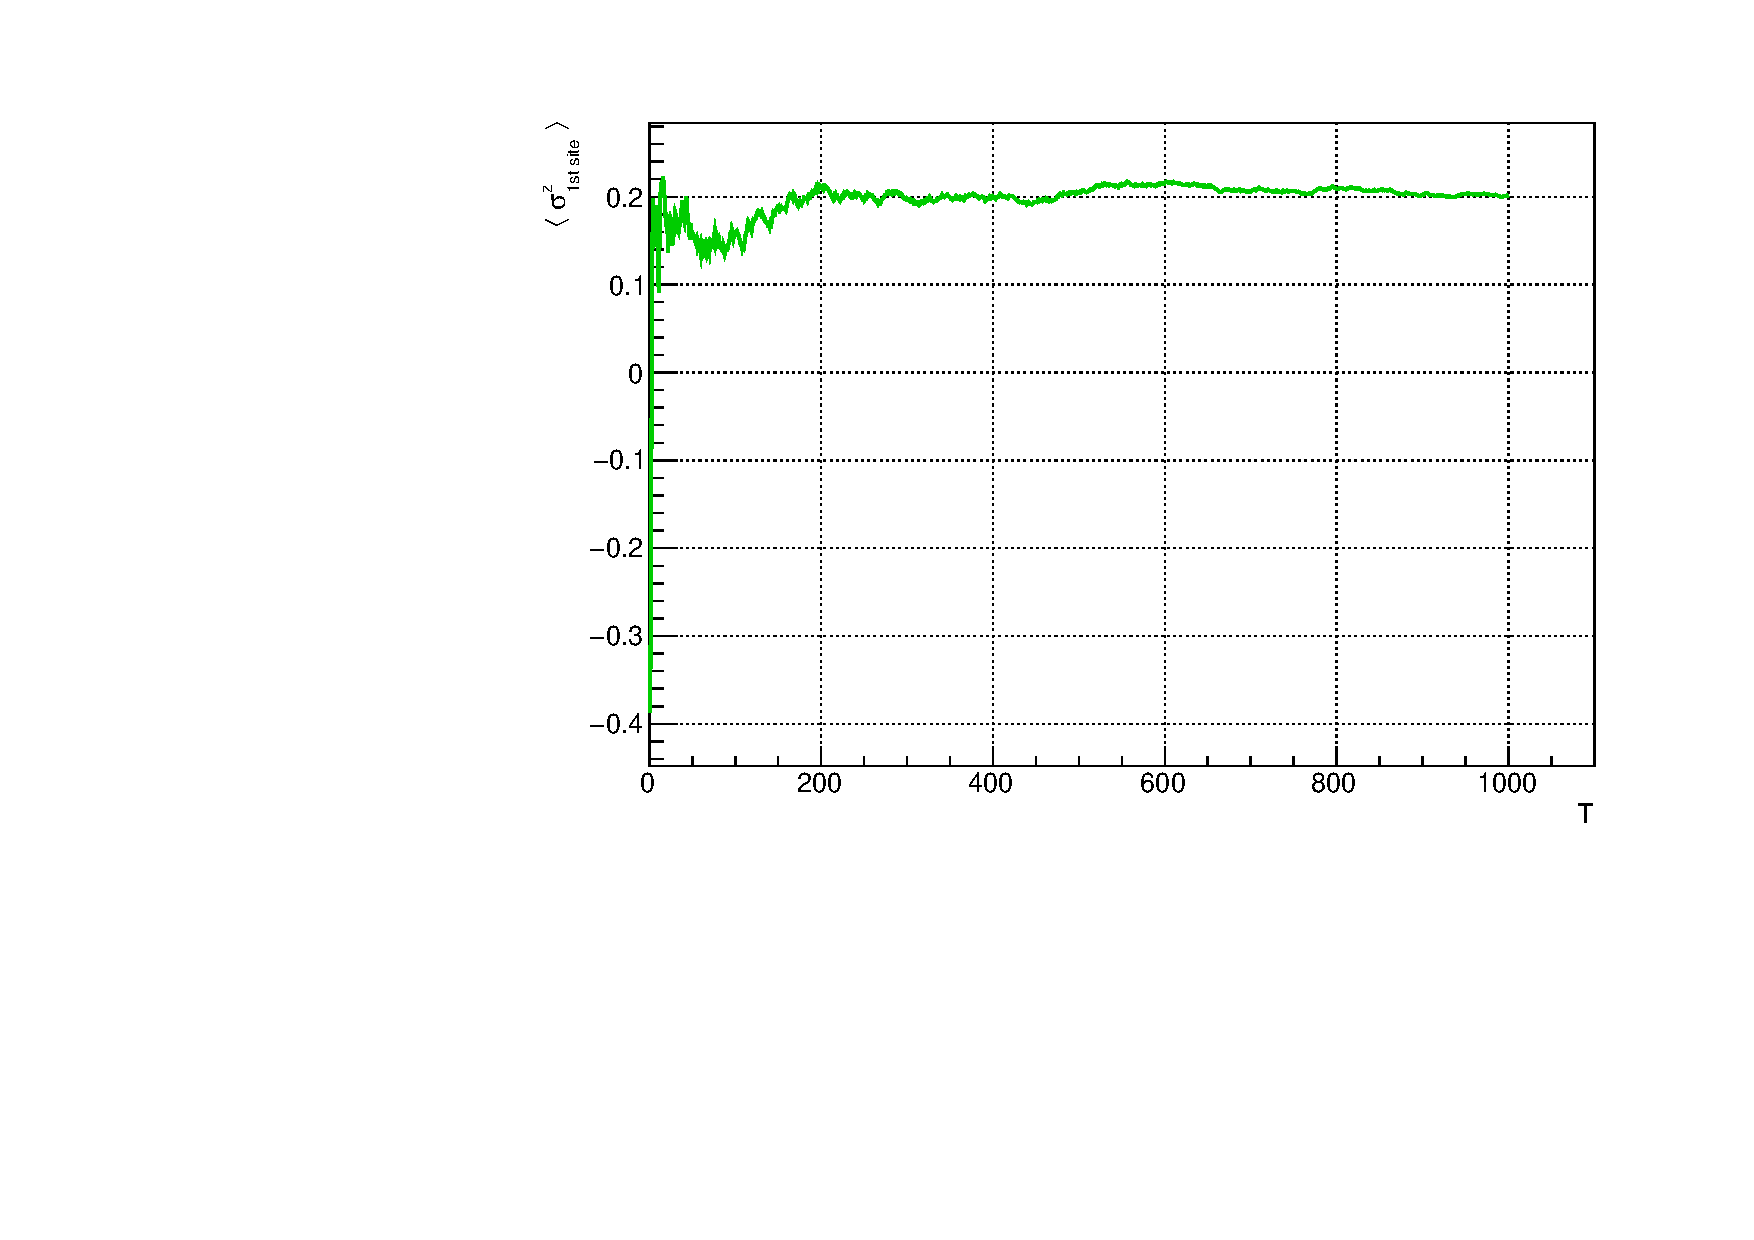
\includegraphics[scale=0.7]{Figures/convergence/Convergence_s8J10505.pdf}
    \caption{Study of convergence of the QT method for a 8-sites chain, for time step $dt=0.1$, T being the whole elapsed time.}
    \label{fig:convergenceMPO_8sites}
\end{figure}

\begin{figure}[H]
    \centering
    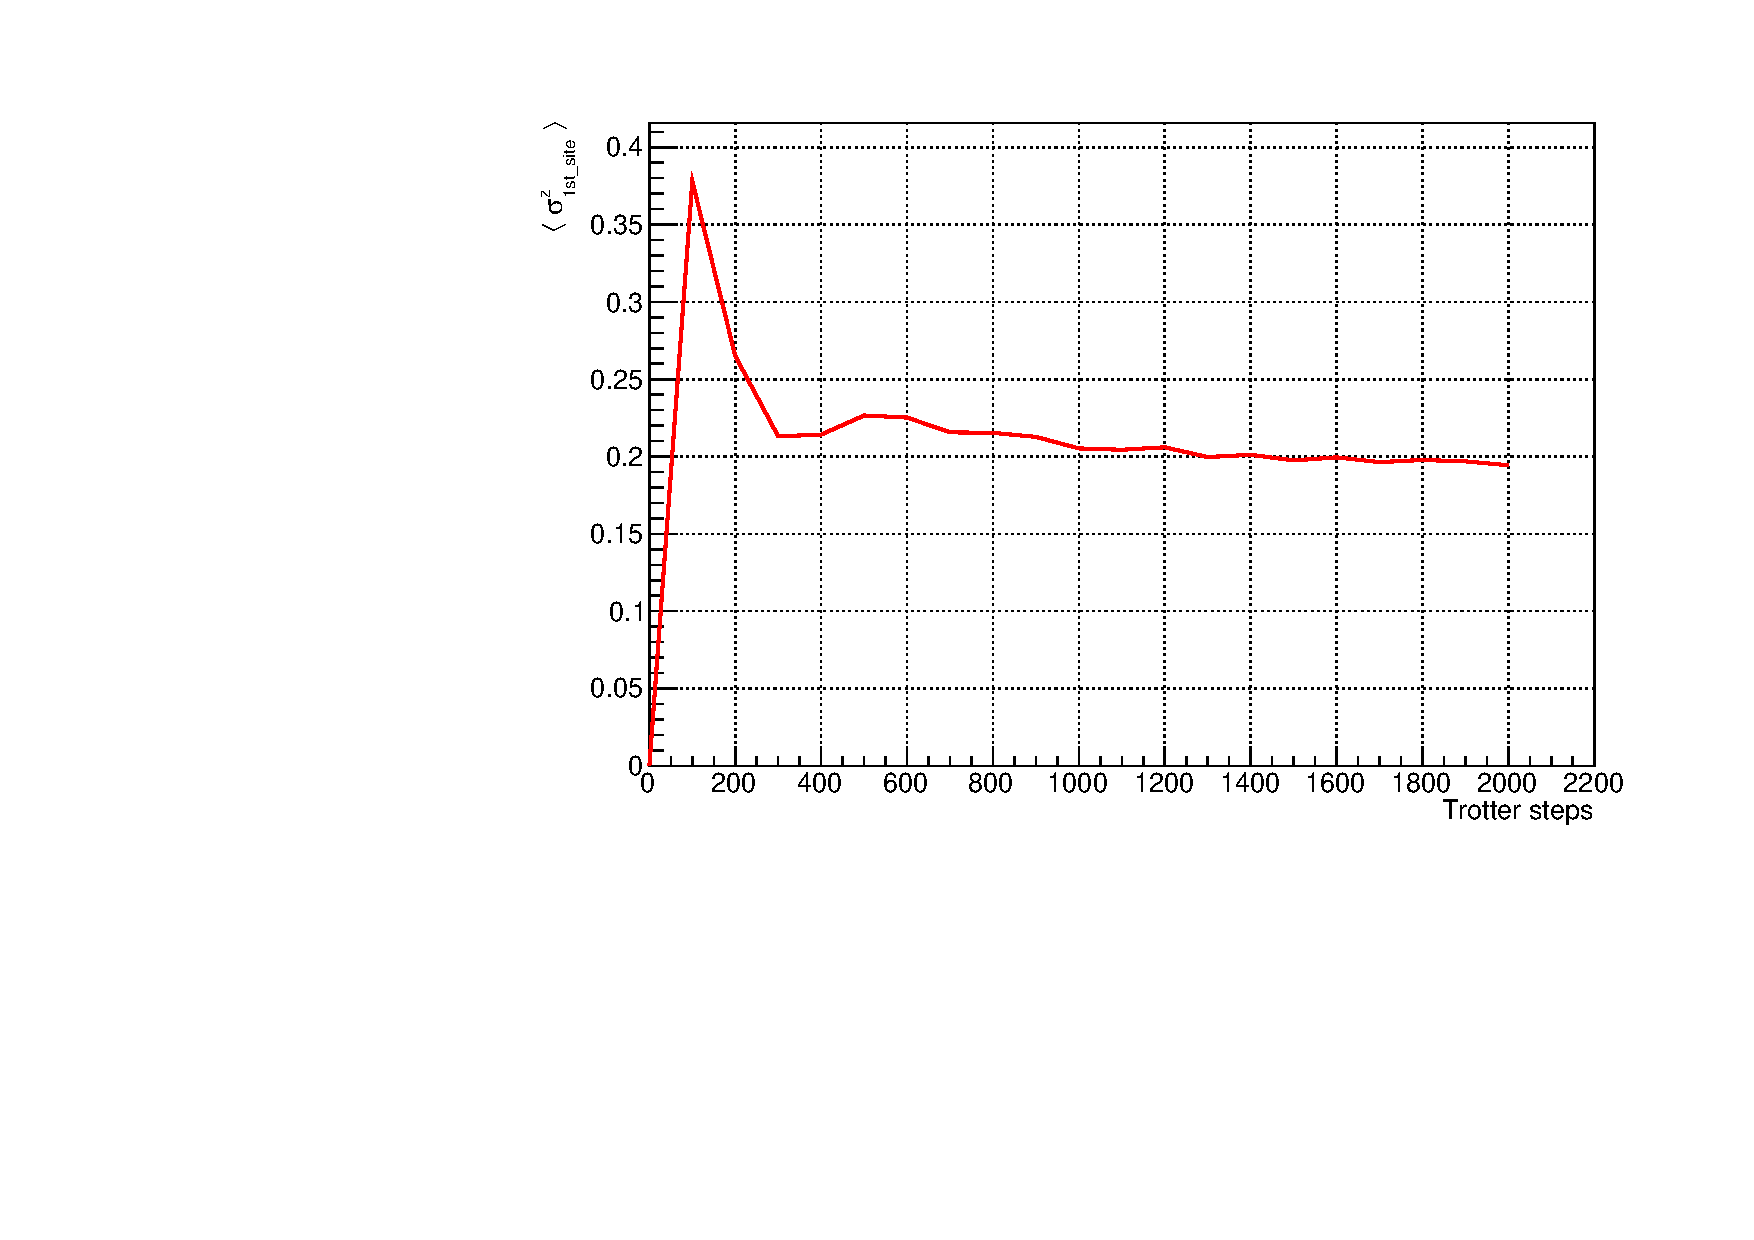
\includegraphics[scale=0.7]{Figures/12sites/ConvergenceLML012m060Time002000_J10505.pdf}
    \caption{Study of convergence of the MPO method for a 12-sites chain, for bond dimension m = 60 and T = 2000.}
    \label{fig:my_label}
\end{figure}

\begin{figure}[H]
    \centering
    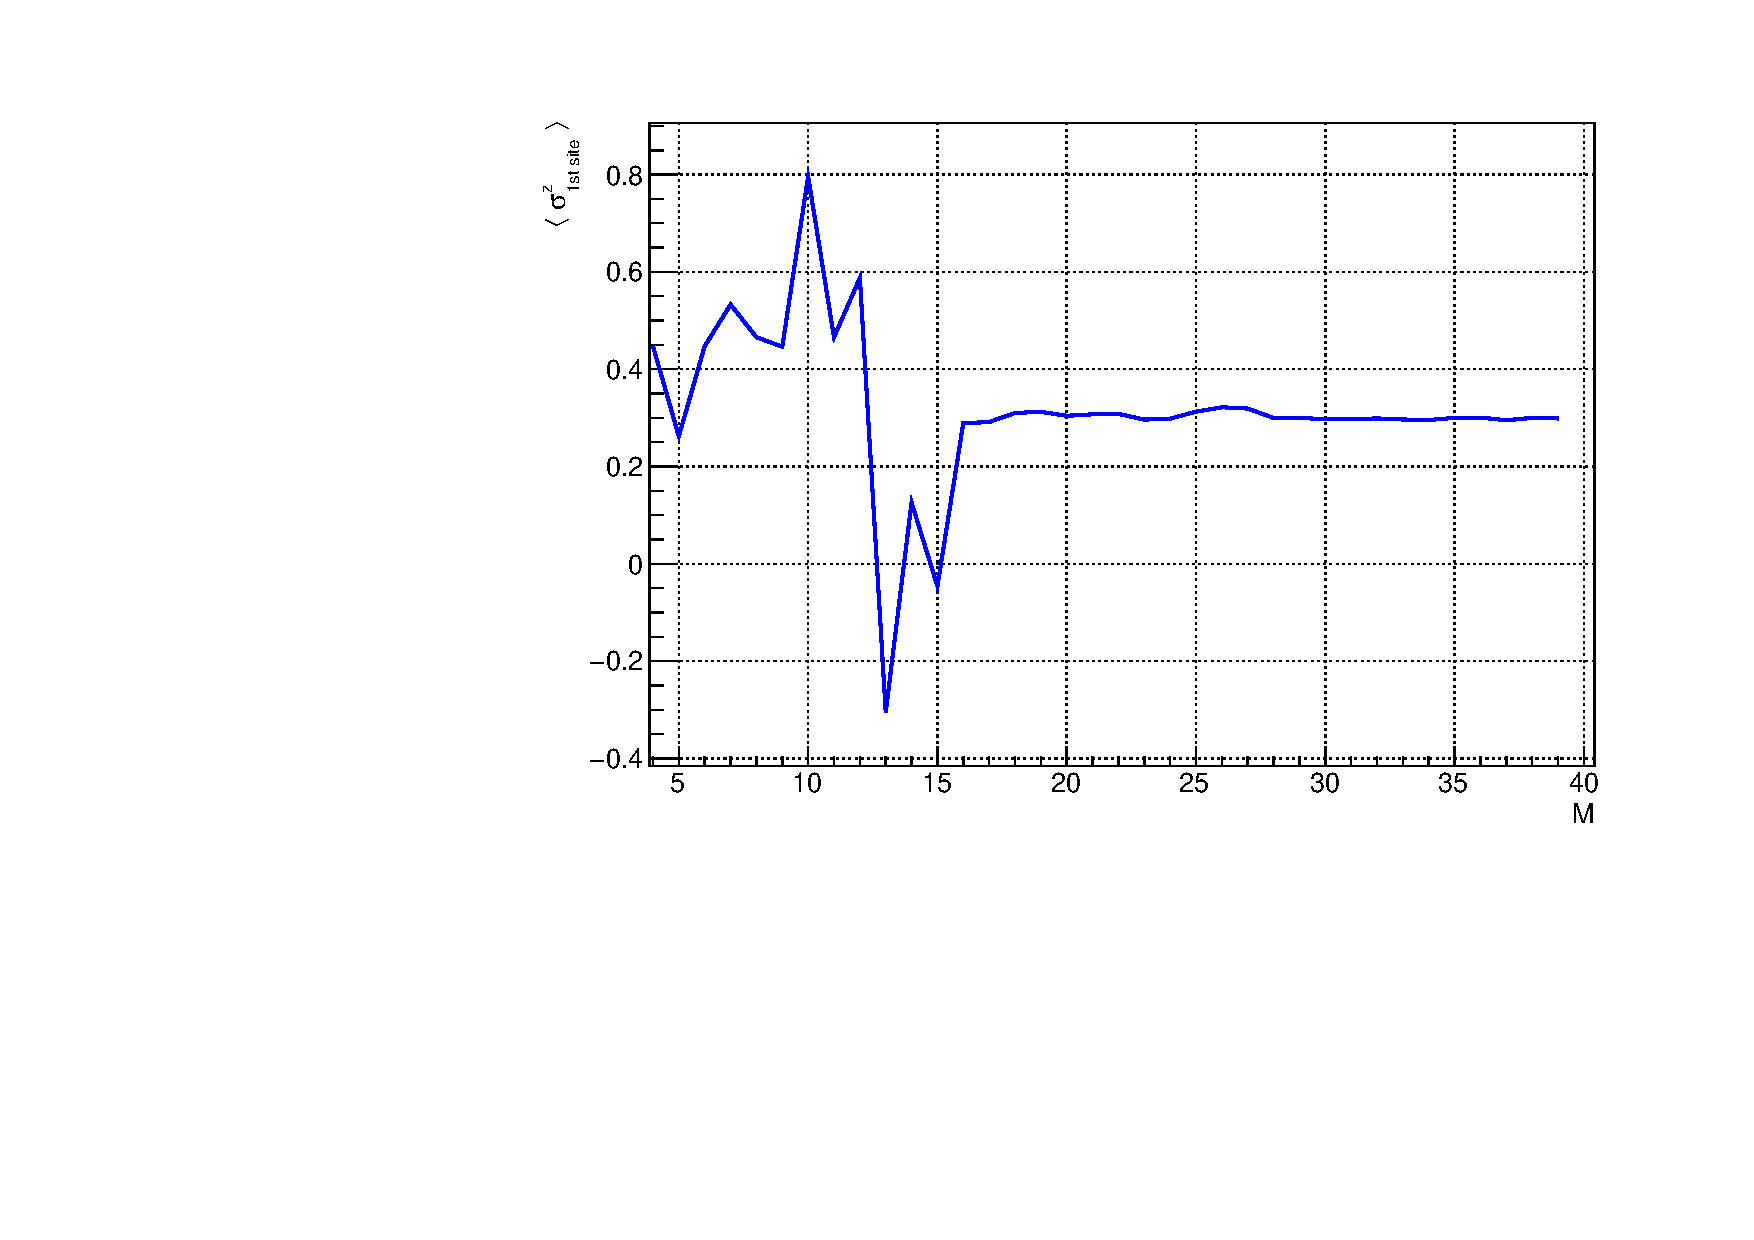
\includegraphics[scale=0.7]{Figures/convergence/s16_M40J10505_Convergence.pdf}
    \caption{Study of convergence of the CSR method for a 16-sites chain, with corner size $M=40$.}
    \label{fig:my_label}
\end{figure}

\textcolor{red}{ERRORS?}

\section{Magnetization Profile}
The first observable we are going to examine is the magnetization profile of the chain, i.e. the expectation value $\langle \sigma^z \rangle$ of the Pauli spin- matrix $\sigma^z$ for each site. 

\begin{figure}[H]
    \centering
    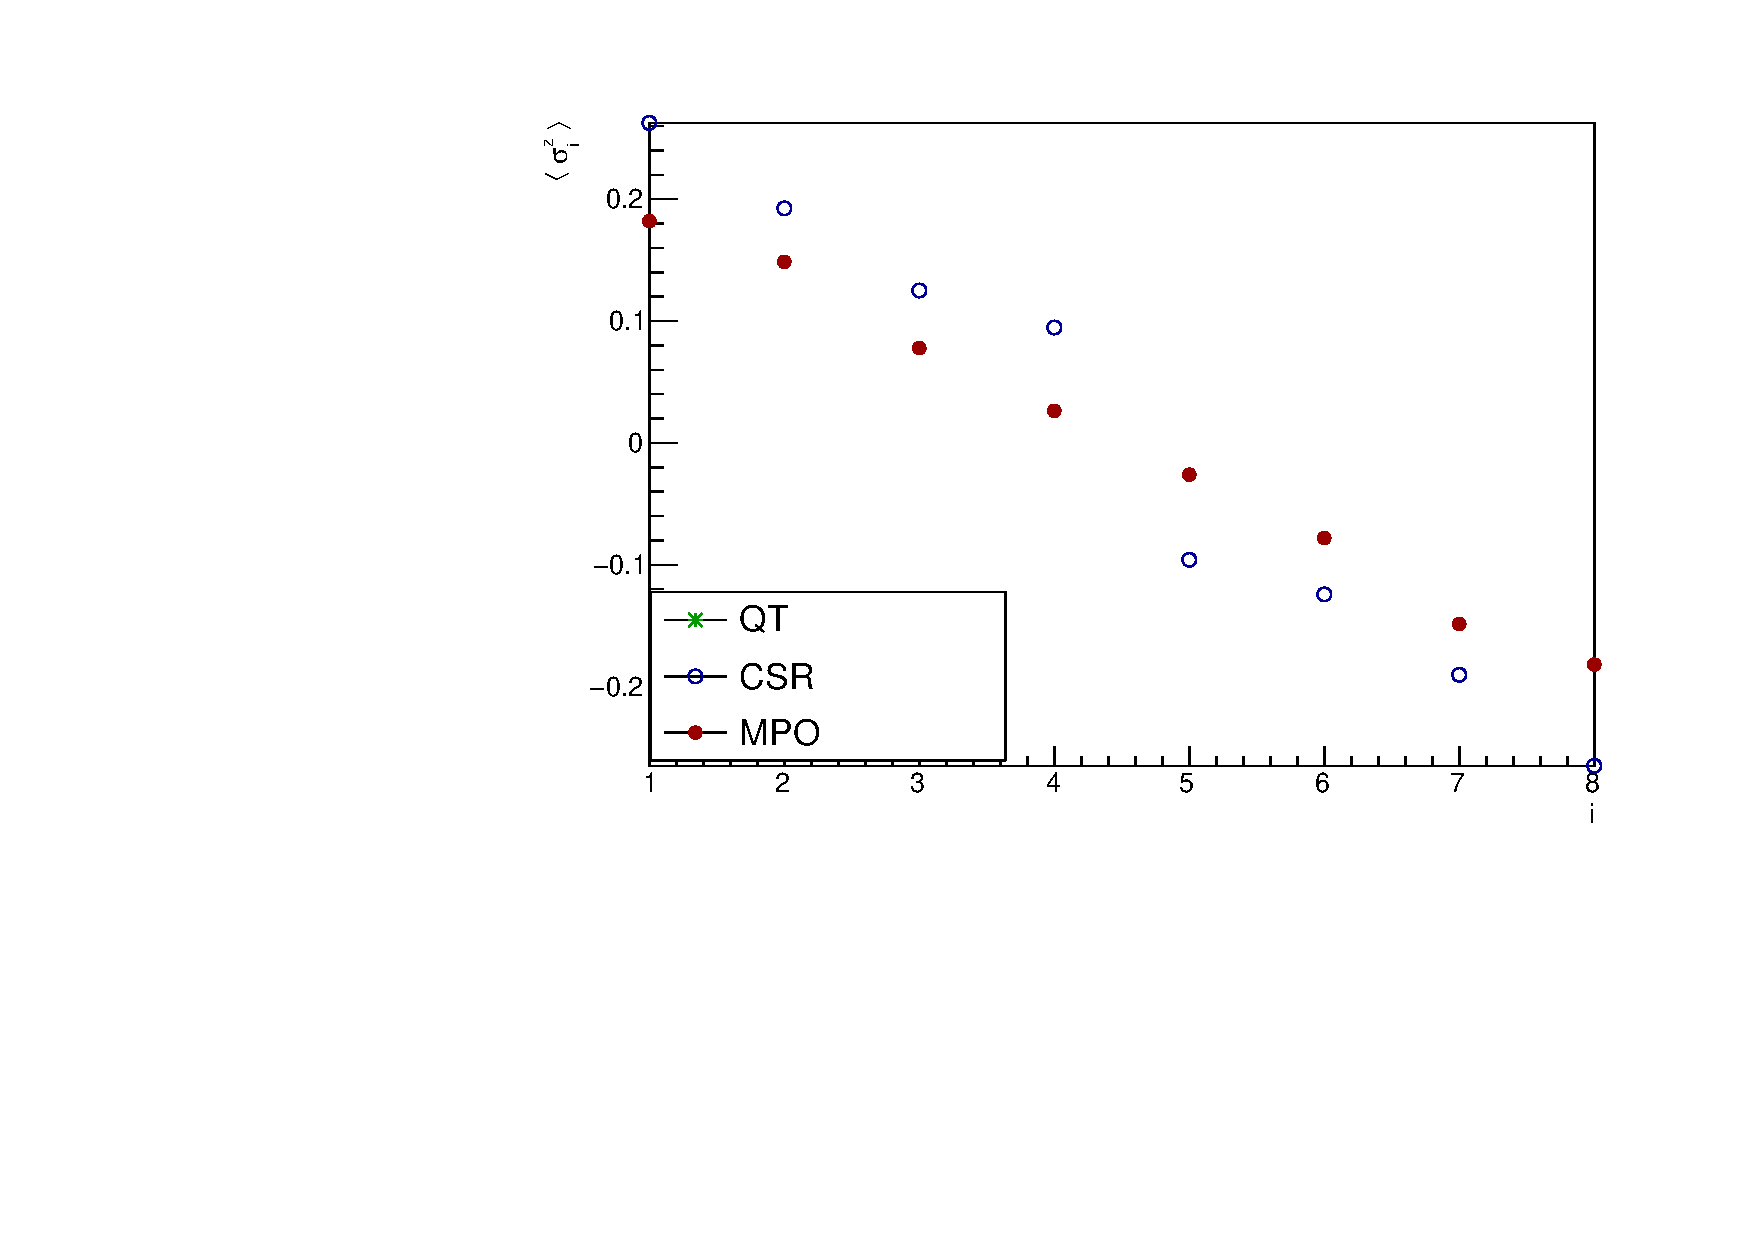
\includegraphics[scale=0.7]{Figures/8sites_comparison/LMComparison_8sJ10505.pdf}
    \caption{Spin profile for a 8-sites chain characterized by $\gamma~=~1, J_x=1, J_y=0.5, J_z=0.5$; \emph{i} stands for the site index.}
    \label{fig:8sites_LMcomparisonJz05}
\end{figure}

\begin{figure}[H]
    \centering
    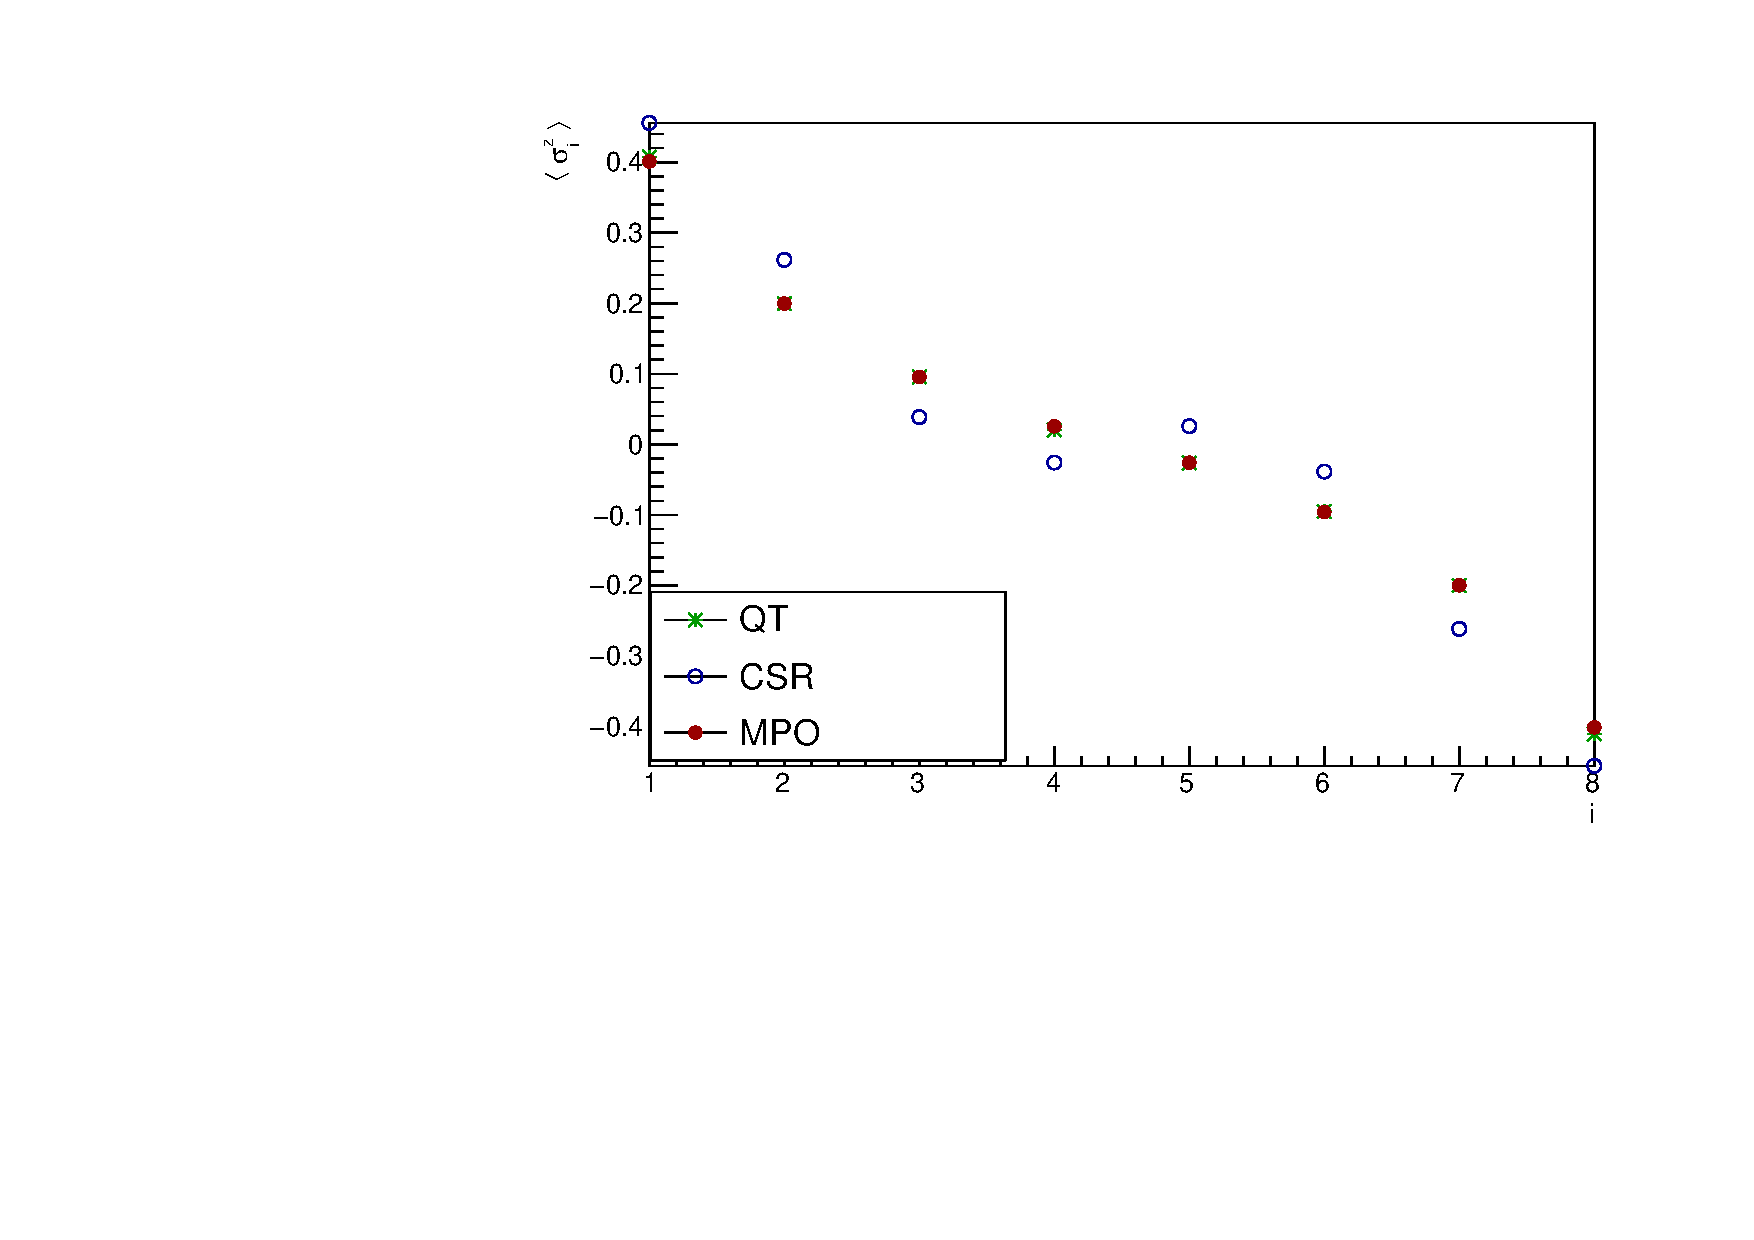
\includegraphics[scale=0.7]{Figures/8sites_comparison/LMComparison_8sJ1051.pdf}
    \caption{Spin profile for a 8-sites chain characterized by $\gamma~=~1, J_x=1, J_y=0.5, J_z=1$; \emph{i} stands for the site index.}
    \label{fig:8sites_LMcomparisonJz1}
\end{figure}

\begin{figure}[H]
    \centering
    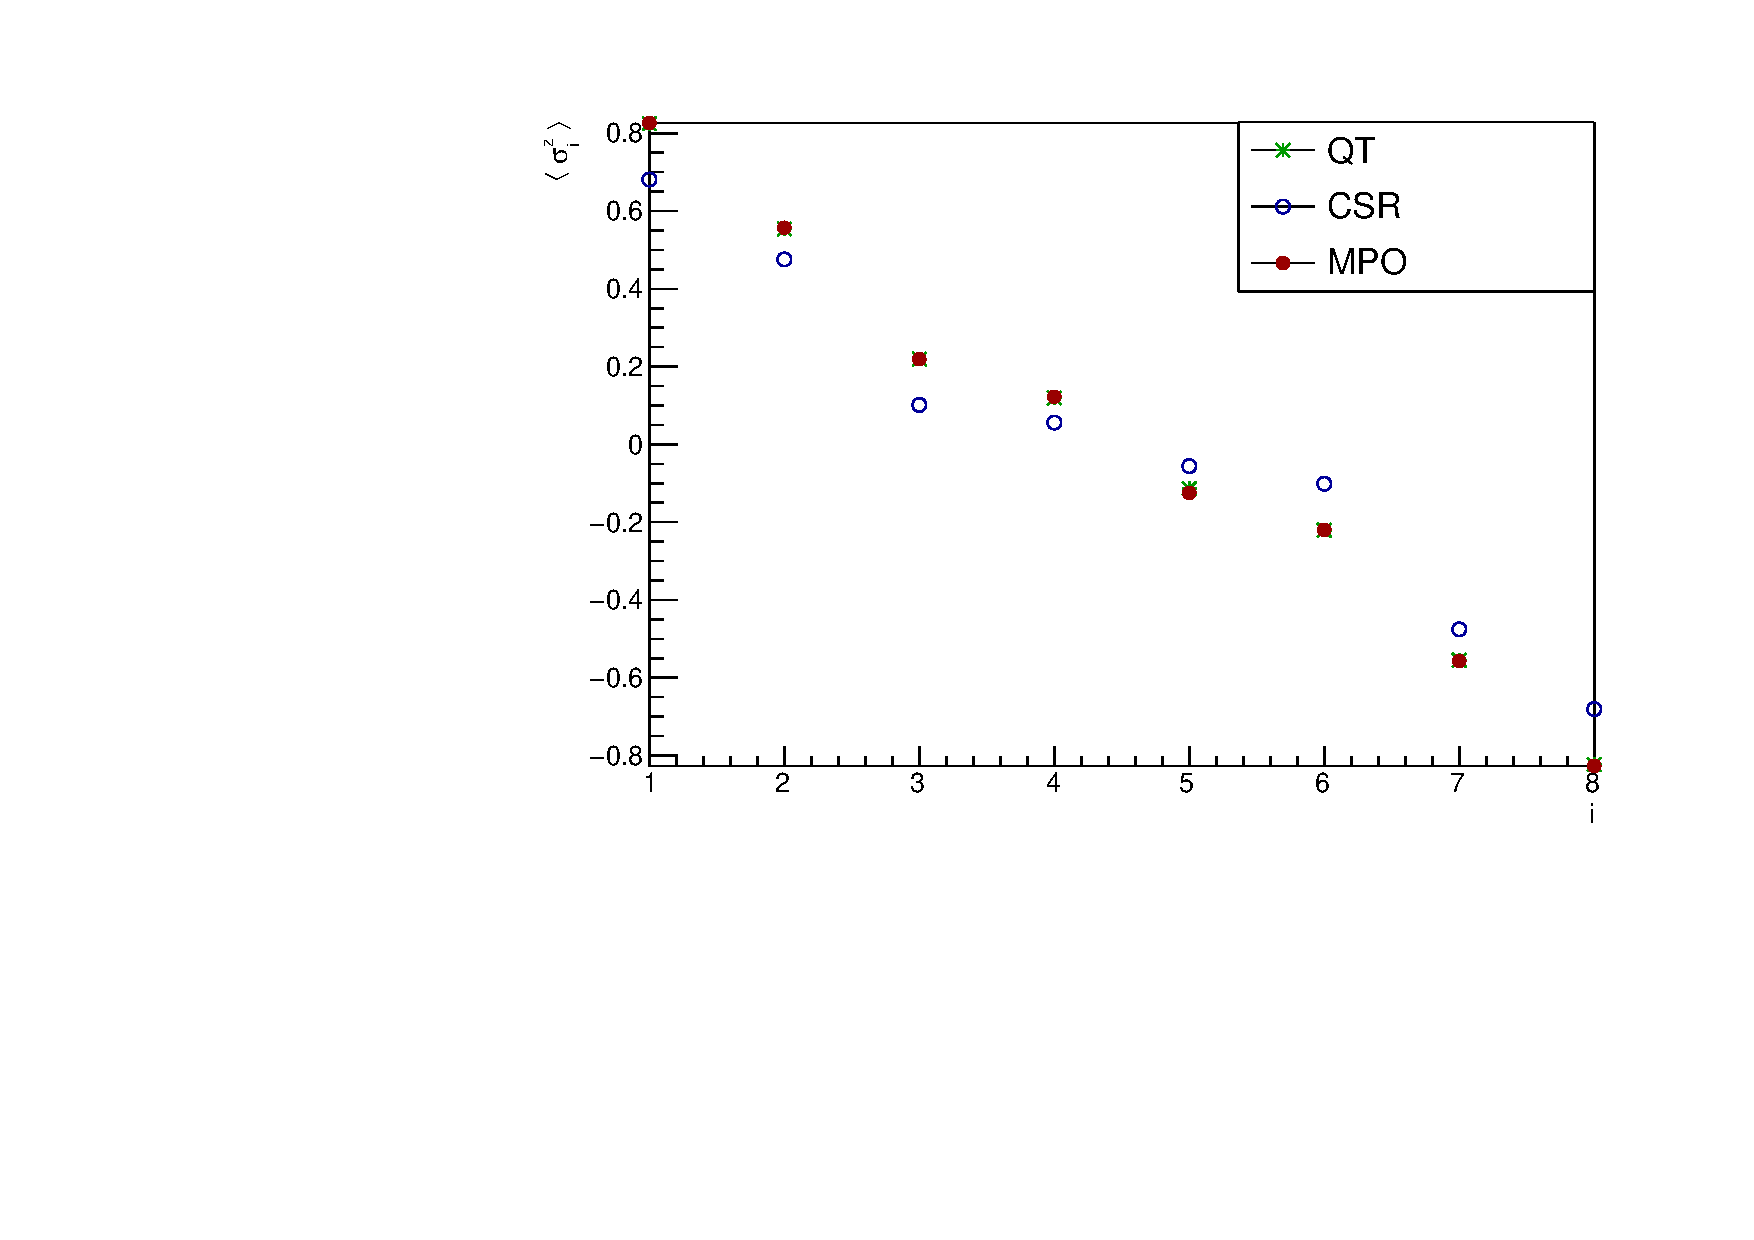
\includegraphics[scale=0.7]{Figures/8sites_comparison/LM_8s_J10515.pdf}
    \caption{Spin profile for a 8-sites chain characterized by $\gamma~=~1, J_x=1, J_y=0.5, J_z=1.5$.}
    \label{fig:my_label}
\end{figure}

It can be interesting seeing if the magnetization changes its profile for different chain lengths; now let us see the case of a \textbf{12-sites} chain for different values of $\Delta$ as done previoulsy. The following data are obtained from MPO method.

\begin{figure}[H]
    \centering
    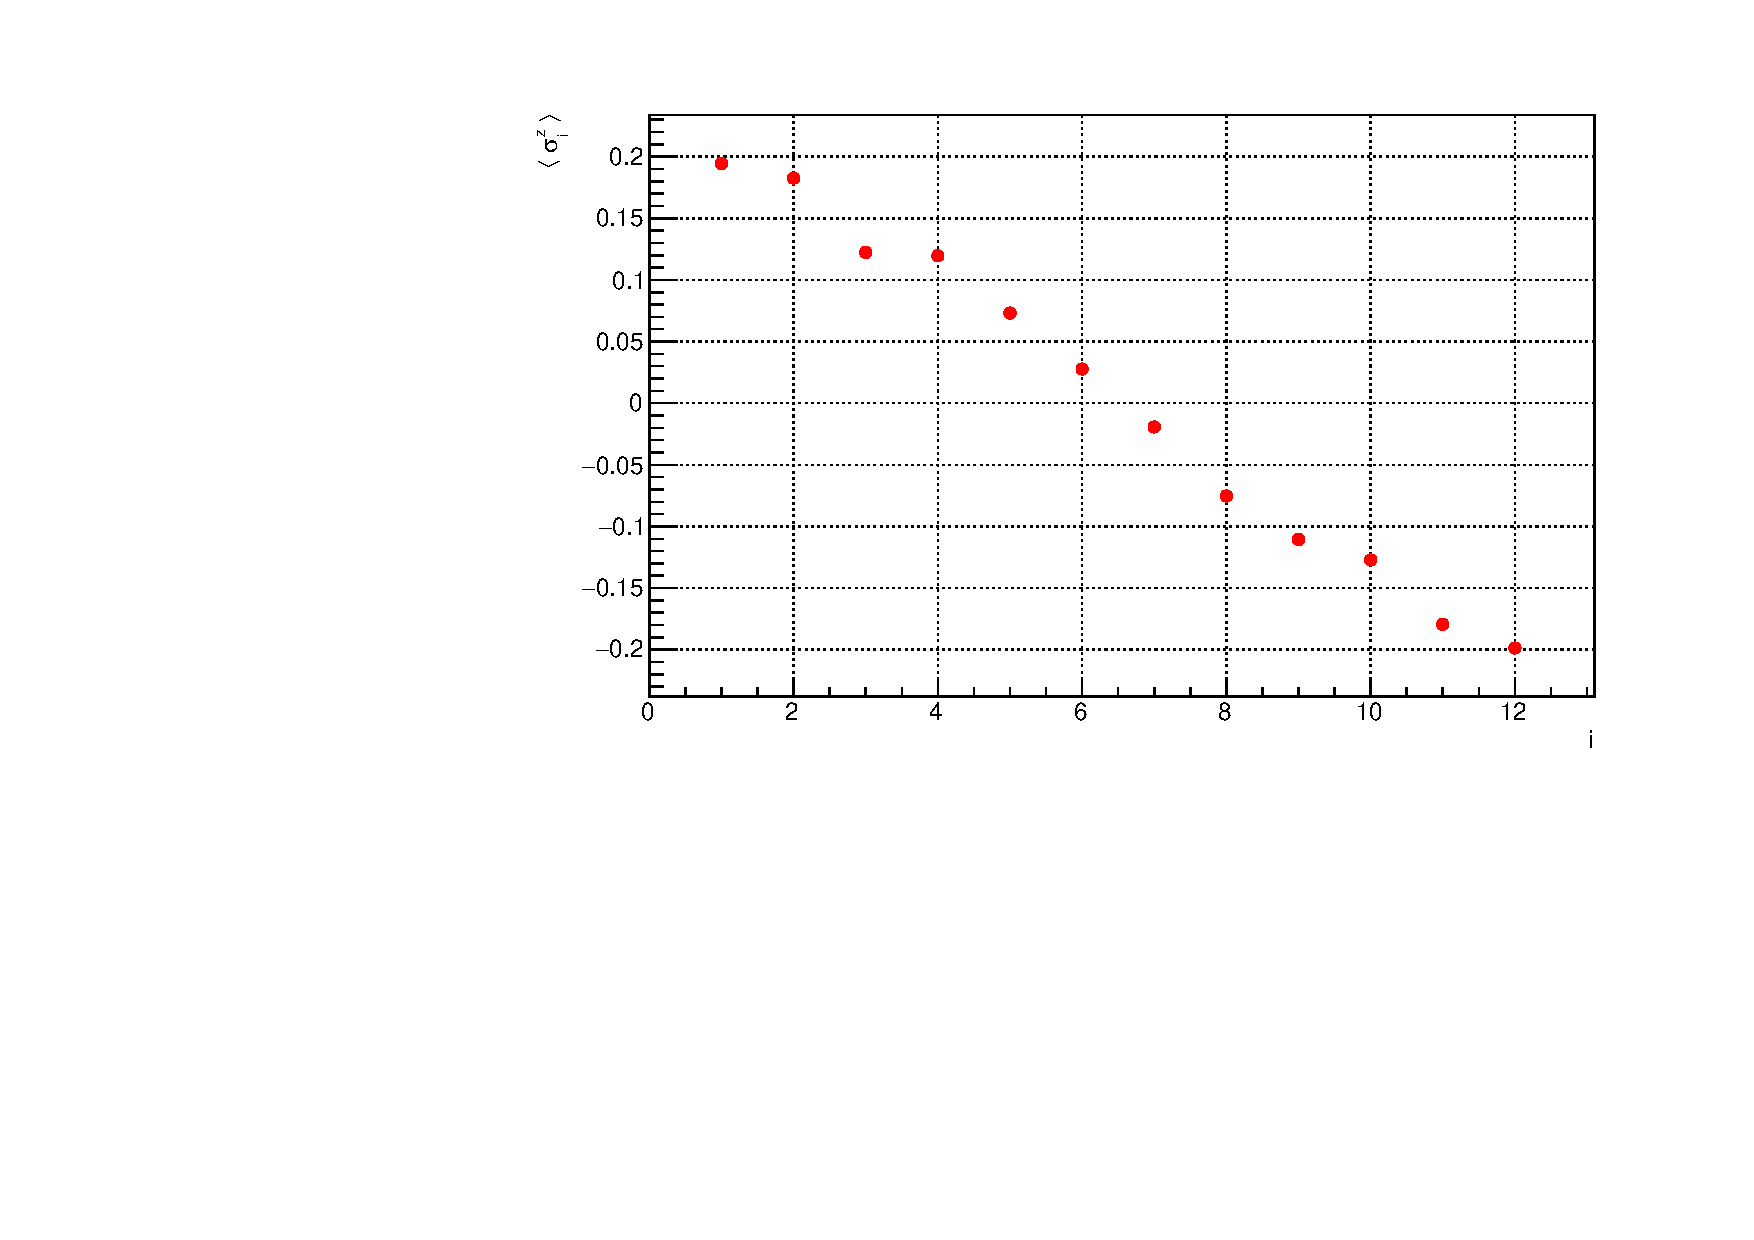
\includegraphics[scale=0.7]{Figures/12sites/LML012m060Time002000_J10505.pdf}
    \caption{Spin profile for a 12-sites chain characterized by $\gamma~=~1, J_x=1, J_y=0.5, J_z=0.5$. Data are obtained from MPO method, with m = 60 and T = 2000.}
    \label{fig:my_label}
\end{figure}

\begin{figure}[H]
    \centering
    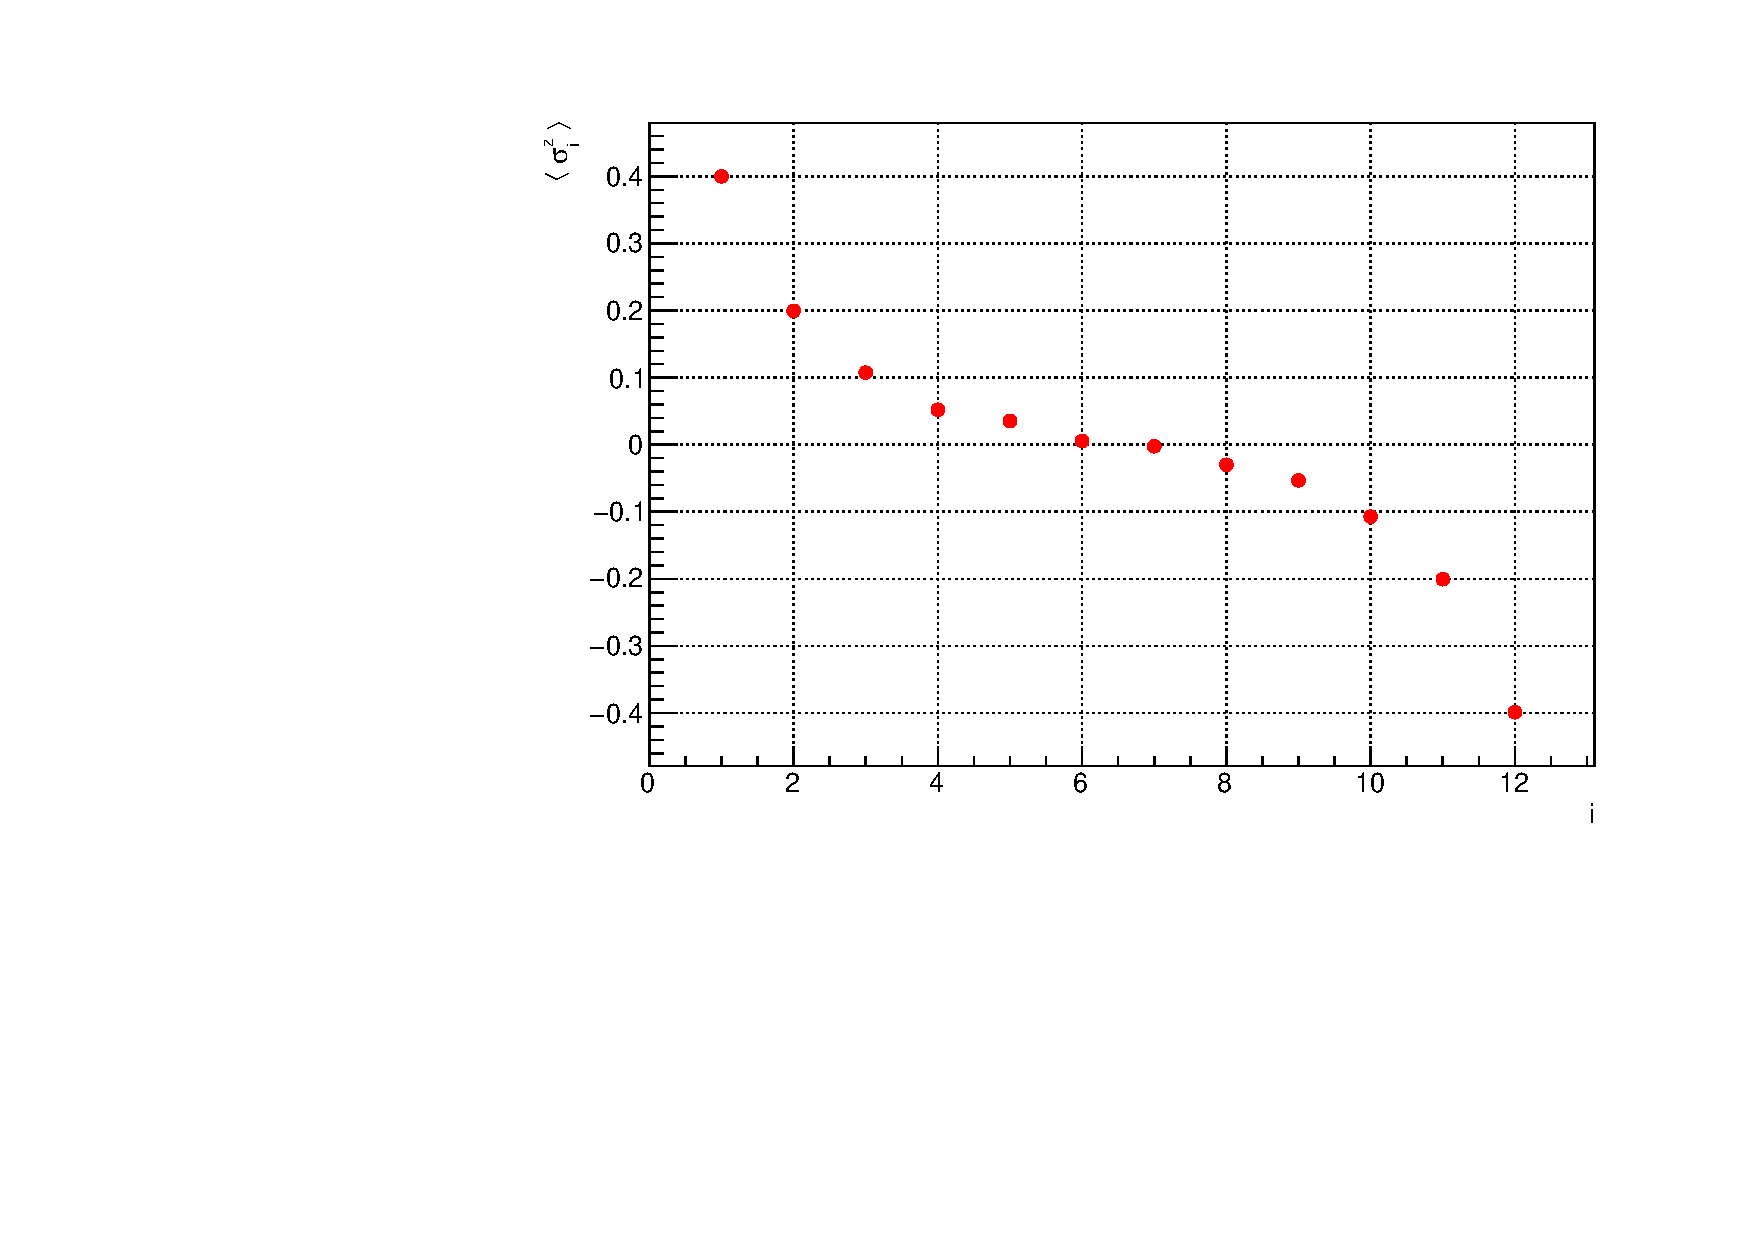
\includegraphics[scale=0.7]{Figures/12sites/LML012m060Time002000_J1051.pdf}
    \caption{Spin profile for a 12-sites chain characterized by $\gamma~=~1, J_x=1, J_y=0.5, J_z=1.$. Data are obtained from MPO method, with m = 60 and T = 2000.}
    \label{fig:my_label}
\end{figure}

\begin{figure}[H]
    \centering
    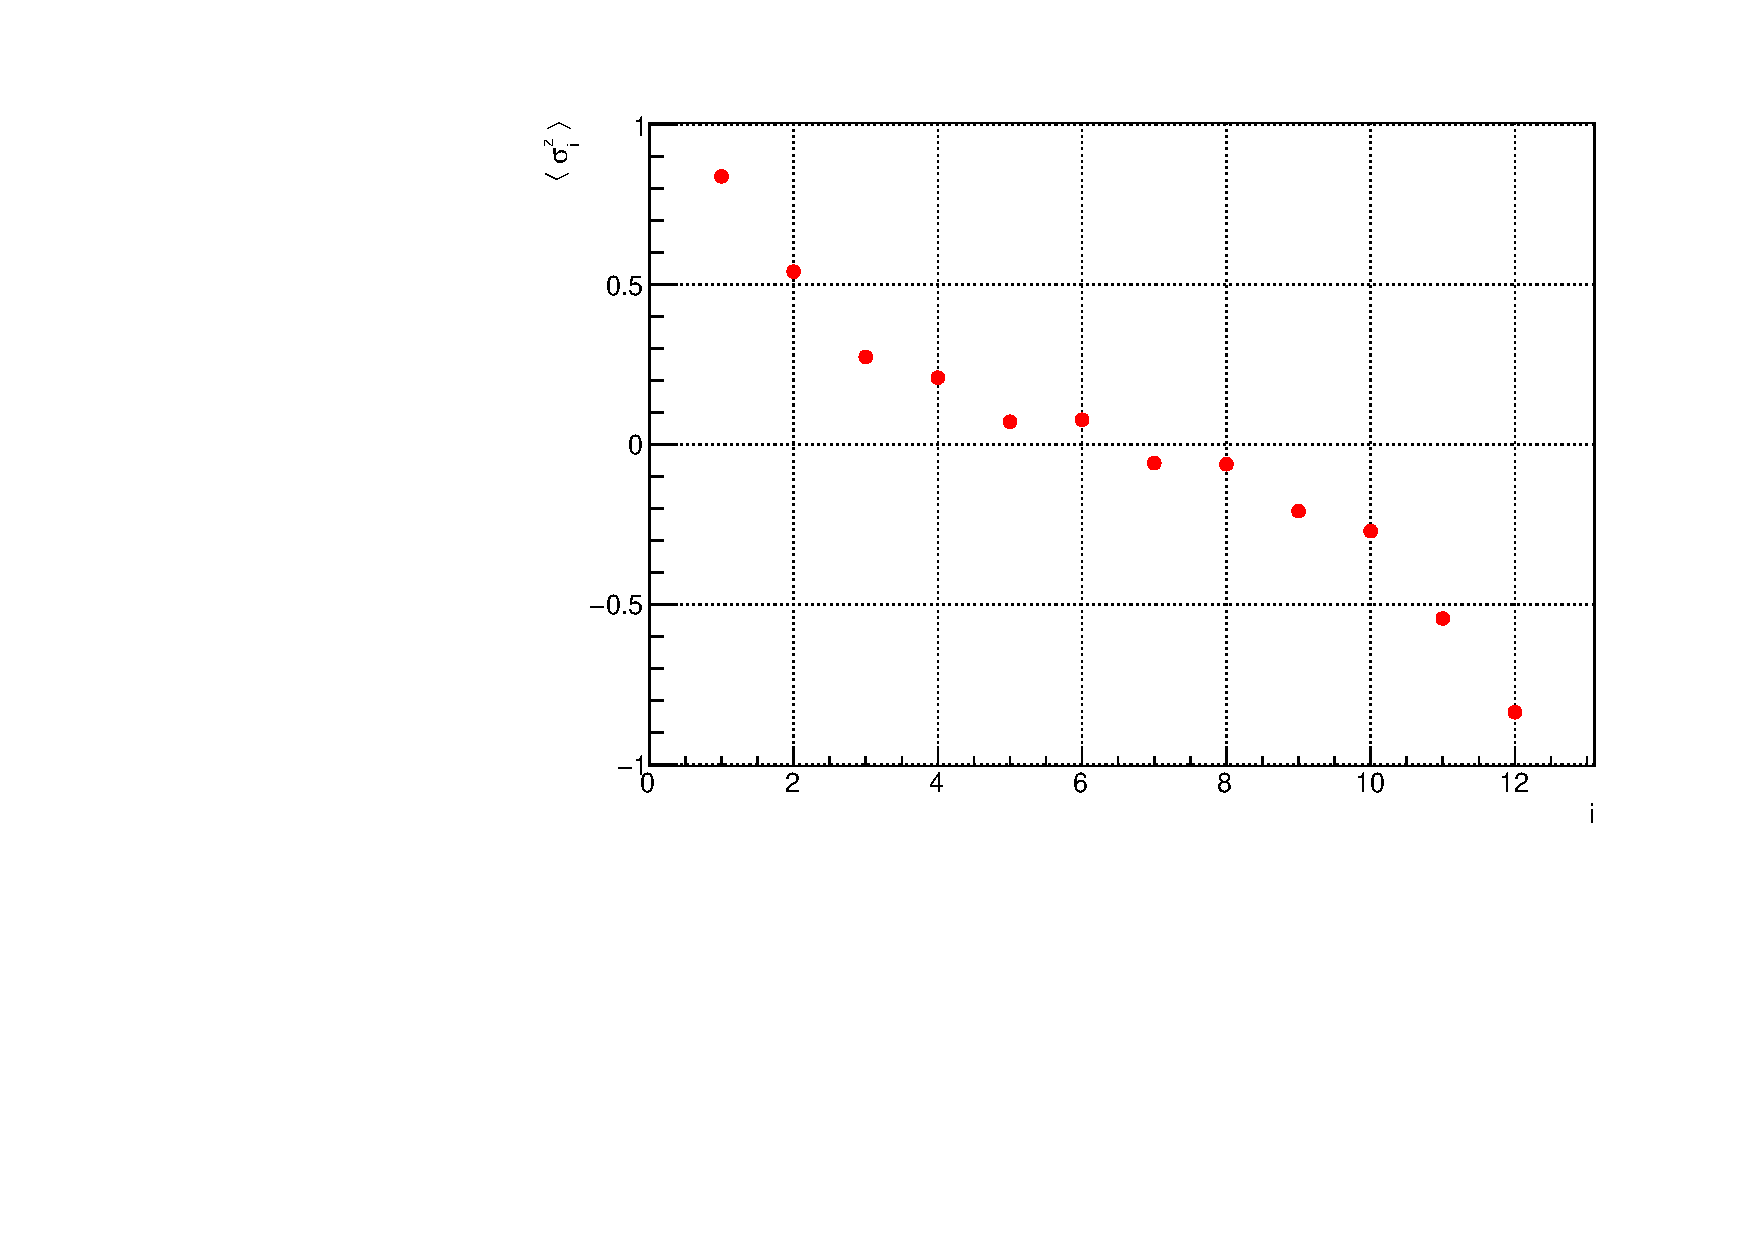
\includegraphics[scale=0.7]{Figures/12sites/LML012m060Time002000_J10515.pdf}
    \caption{Spin profile for a 12-sites chain characterized by $\gamma~=~1, J_x=1, J_y=0.5, J_z=1.5$. Data are obtained from MPO method, with m = 60 and T = 2000.}
    \label{fig:my_label}
\end{figure}

Let us see \textbf{16-sites} chain.

\begin{figure}[H]
    \centering
    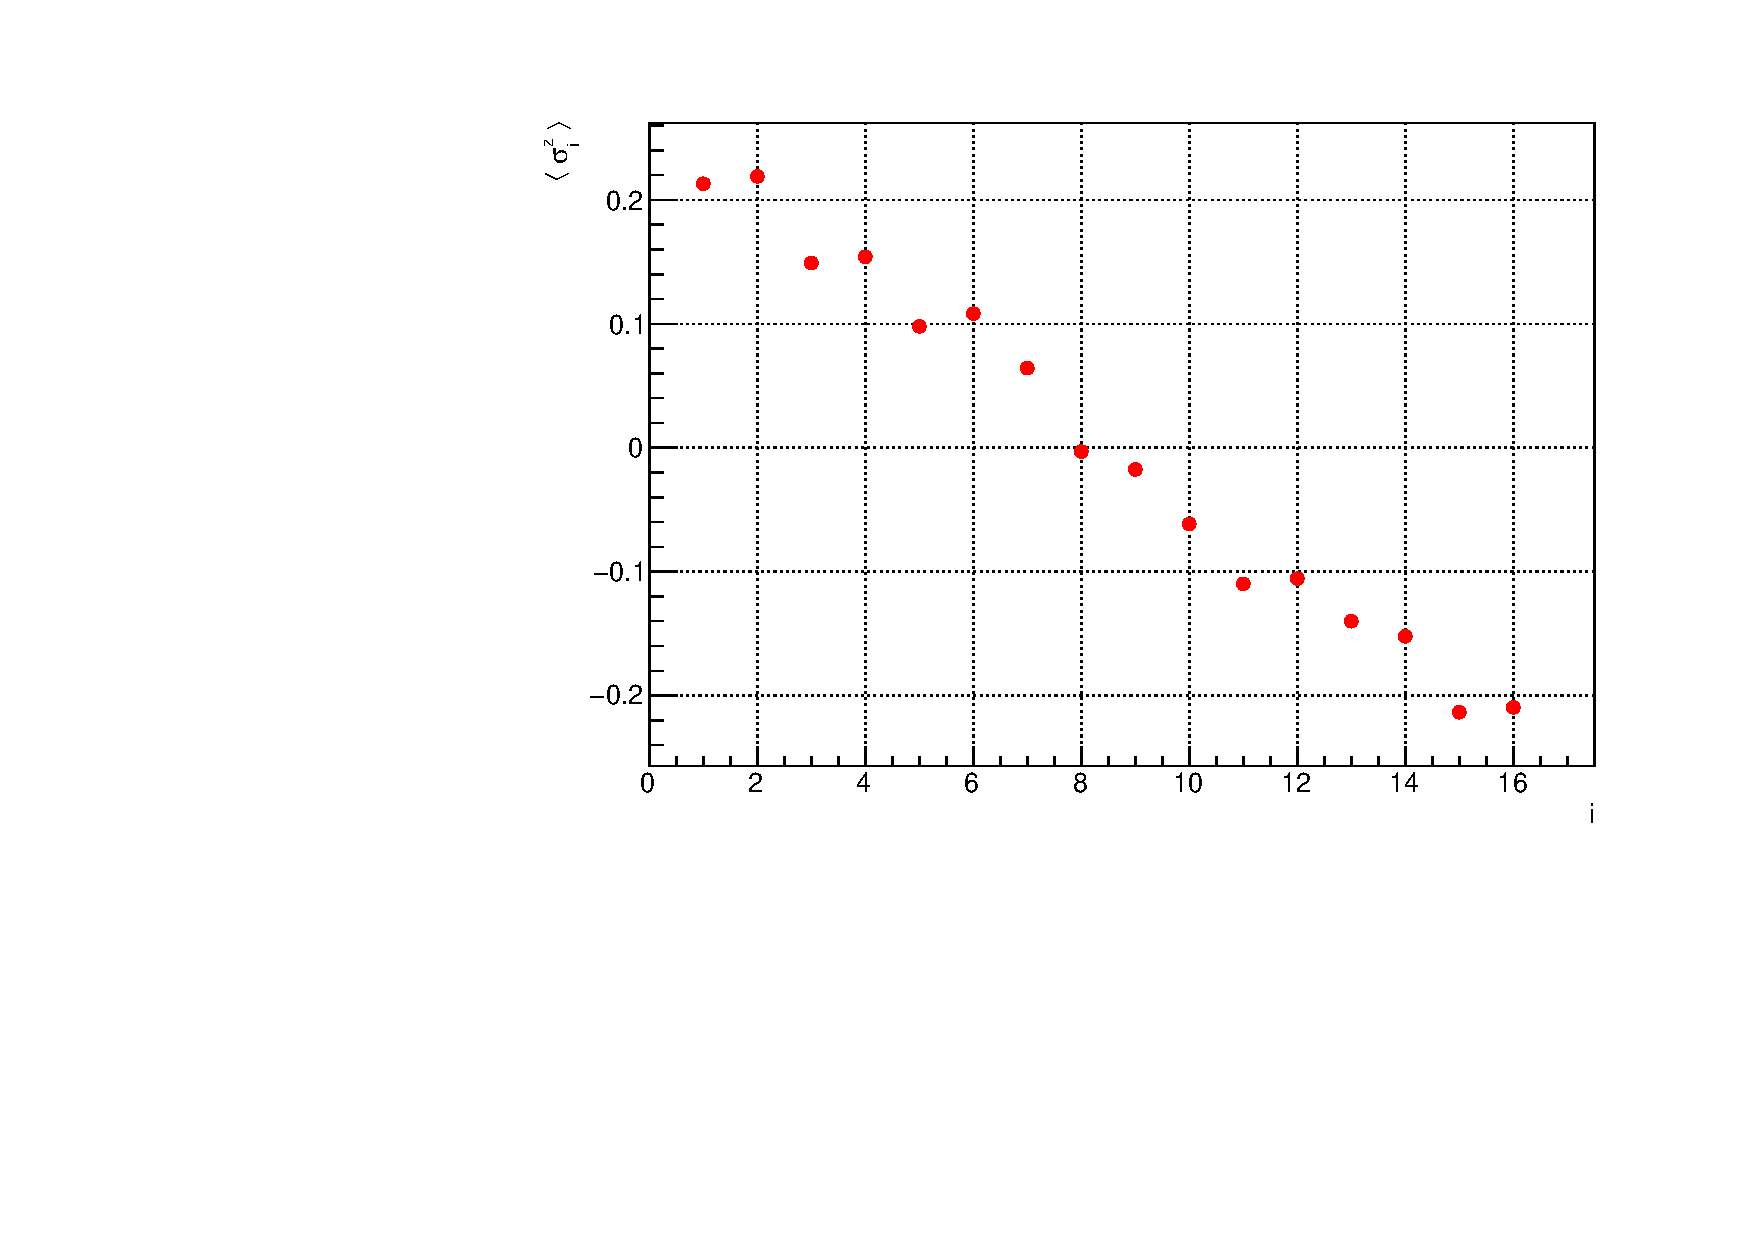
\includegraphics[scale=0.7]{Figures/16sites/LML016m080Time001000_J10505.pdf}
    \caption{Spin profile for a 16-sites chain characterized by $\gamma~=~1, J_x=1, J_y=0.5, J_z=0.5$. Data are obtained from MPO method, with m = 80 and T = 1000.}
    \label{fig:my_label}
\end{figure}

\begin{figure}[H]
    \centering
    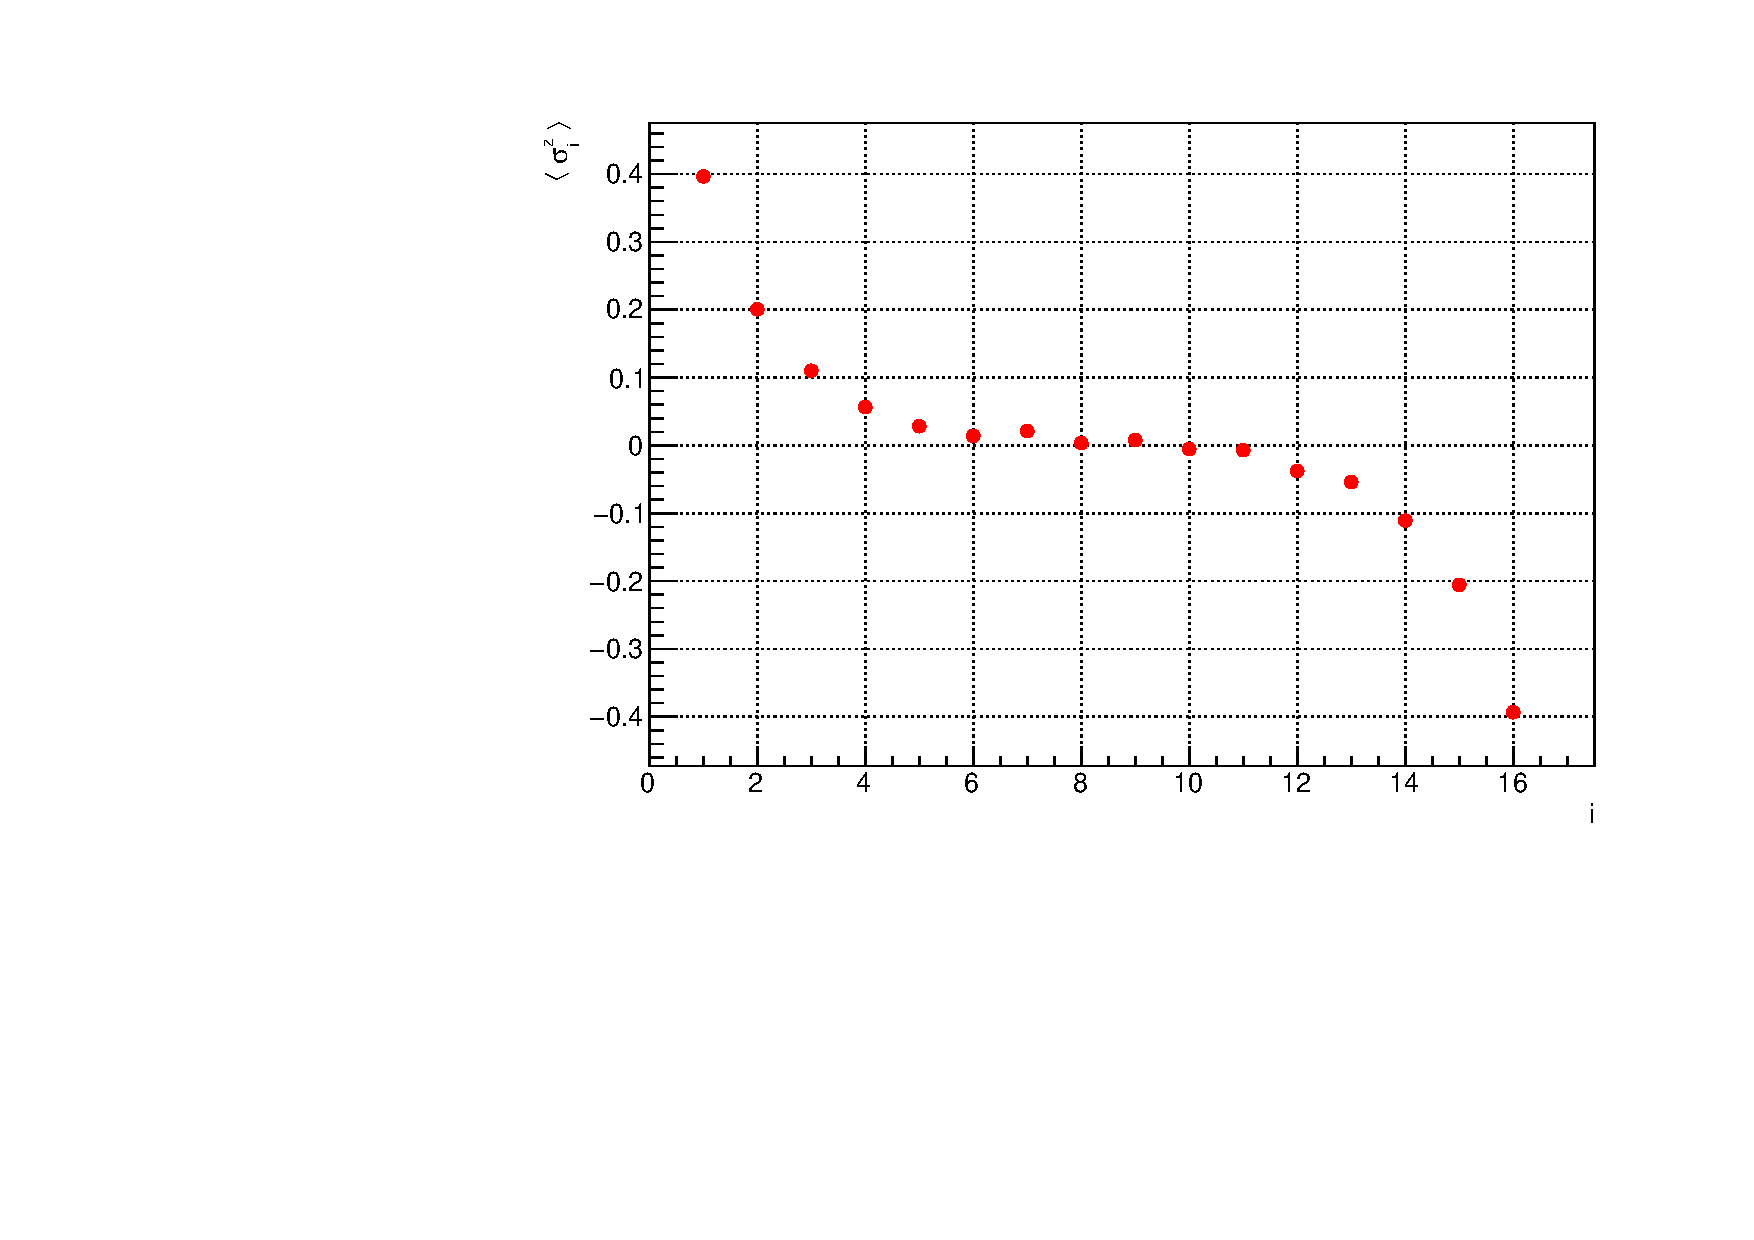
\includegraphics[scale=0.7]{Figures/16sites/LML016m080Time002500_J1051.pdf}
    \caption{Spin profile for a 16-sites chain characterized by $\gamma~=~1, J_x=1, J_y=0.5, J_z=1.$. Data are obtained from MPO method, with m = 80 and T = 2500.}
    \label{fig:my_label}
\end{figure}

\begin{figure}[H]
    \centering
    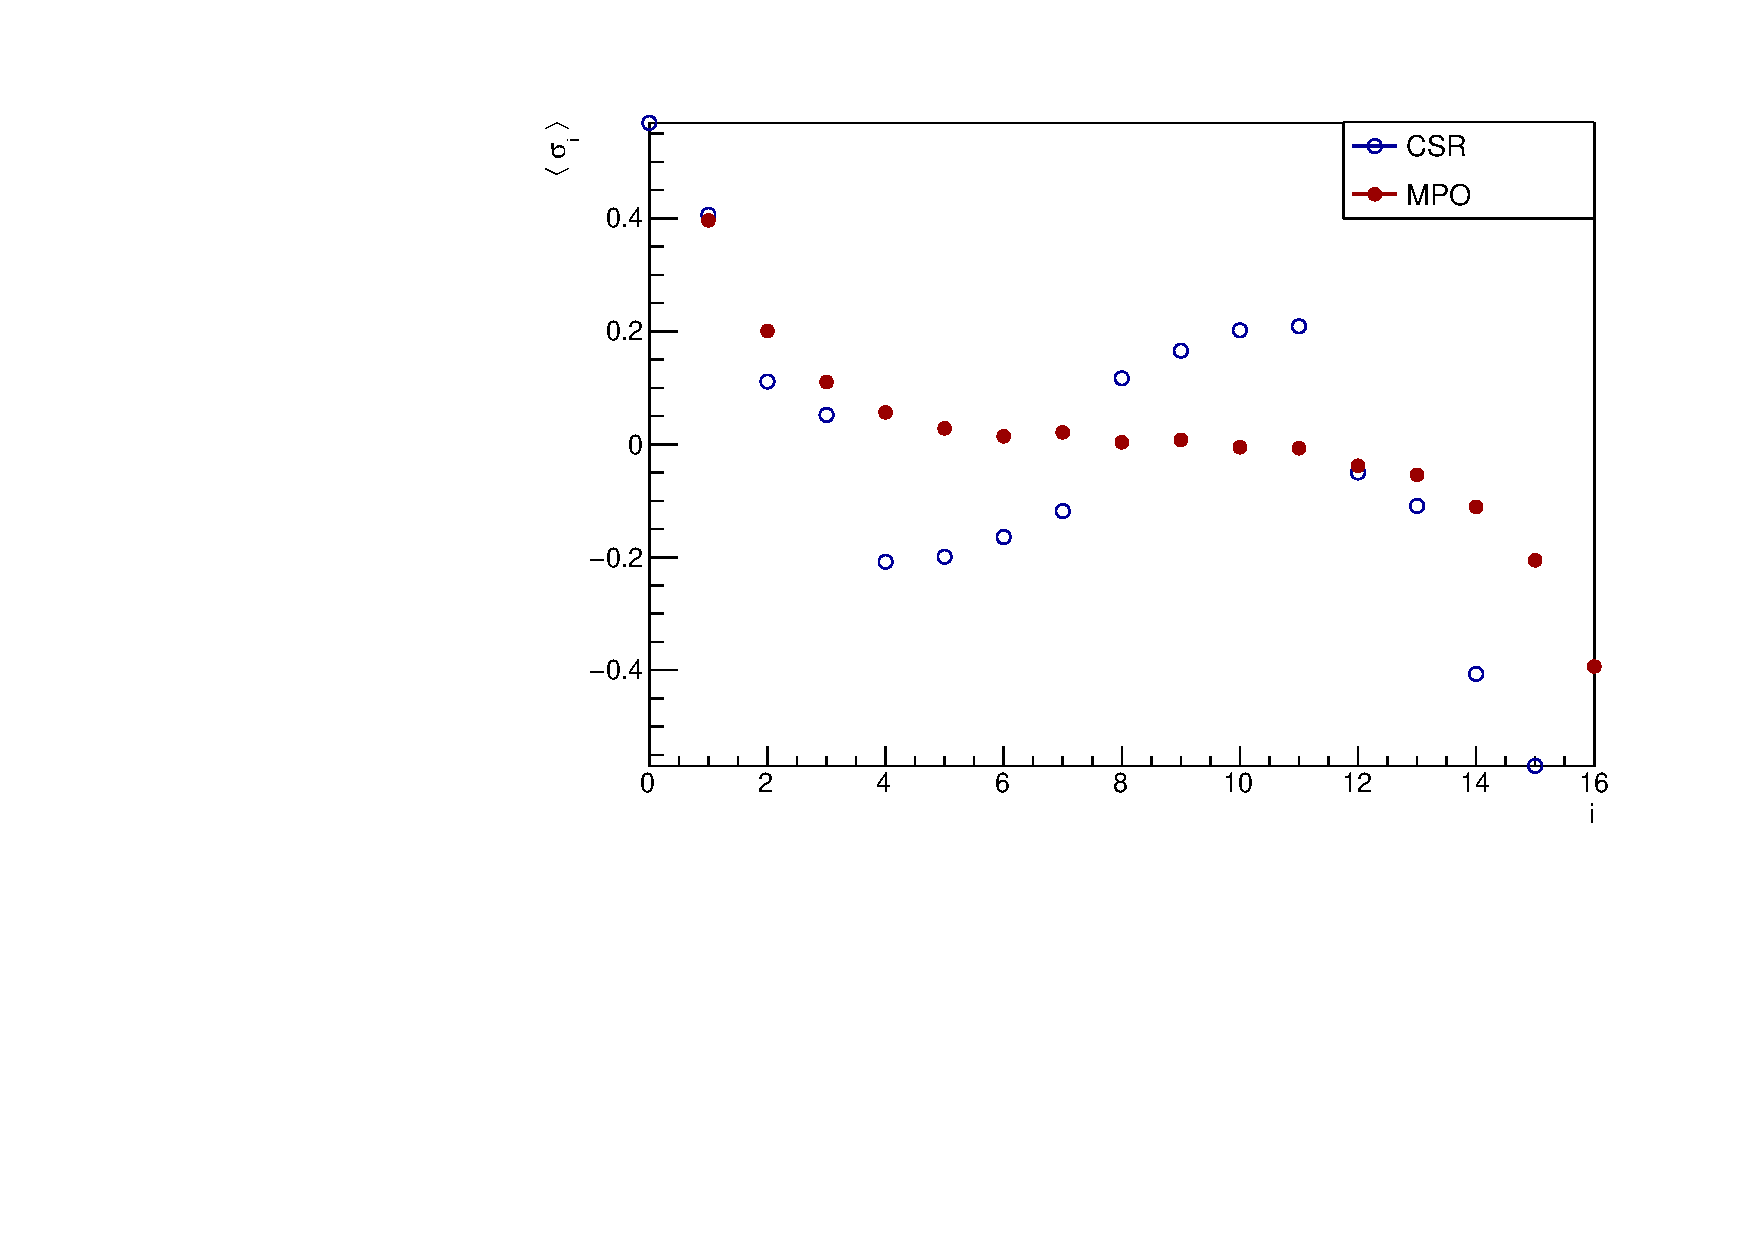
\includegraphics[scale=0.7]{Figures/16sites/LMComparison16s1051.pdf}
    \caption{Spin profile for a 16-sites chain characterized by $\gamma~=~1, J_x=1, J_y=0.5, J_z=1.5$. Data in red are obtained from MPO method, with m = 80 and T = 2000 and data in blue are obtained from CSR method, with M = 40. It is self-evident the inadequacy of the corner-space size: the complete Hilbert space for such a system has a dimension of $2^{16} \times 2^{16}$.}
    \label{fig:my_label}
\end{figure}

The following figure shows the spin profile for the model at $J_z = 1$. 

\textcolor{red}{32-sites chain is missing.}

\begin{figure}[H]
    \centering
    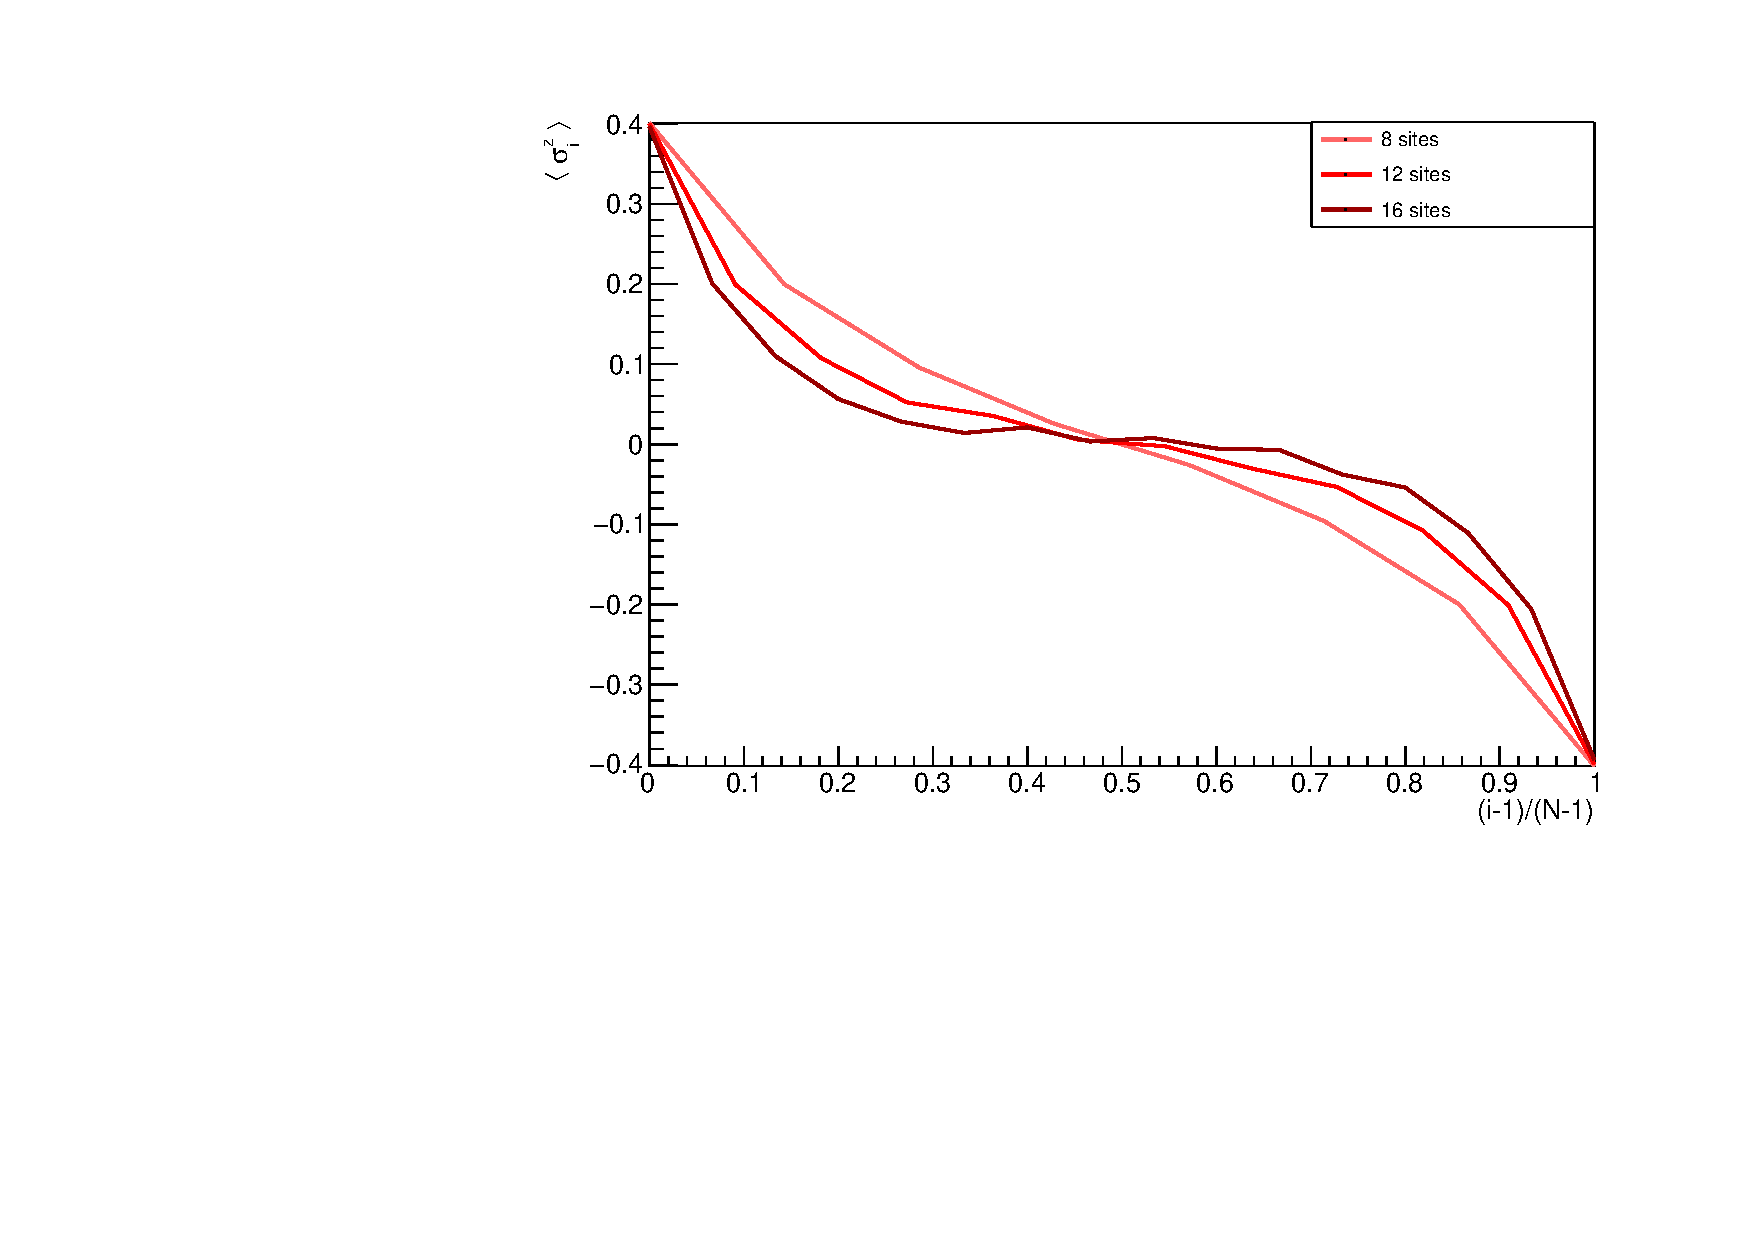
\includegraphics[scale=0.7]{Figures/NORM_LM_comparisonVSsize.pdf}
    \caption{Spin profile for the model under study at $J_z$. Data for different chain length are shown and they are obtained from MPO method.}
    \label{fig:my_label}
\end{figure}


\section{Two-Points Correlation Functions}
As said previously, we are interested in the behaviour of the spins in the chain and how much they are influenced by the presence of the others. In order to analyze this aspect, we are going to study the two-point correlation function with respect to the first and the last site and the \emph{bulk} correlation function.

First of all, as done in the last section, let us see if the results of each method retrace the ones of the other two, for the case of 8-sites chain. 

\begin{figure}[H]
    \centering
    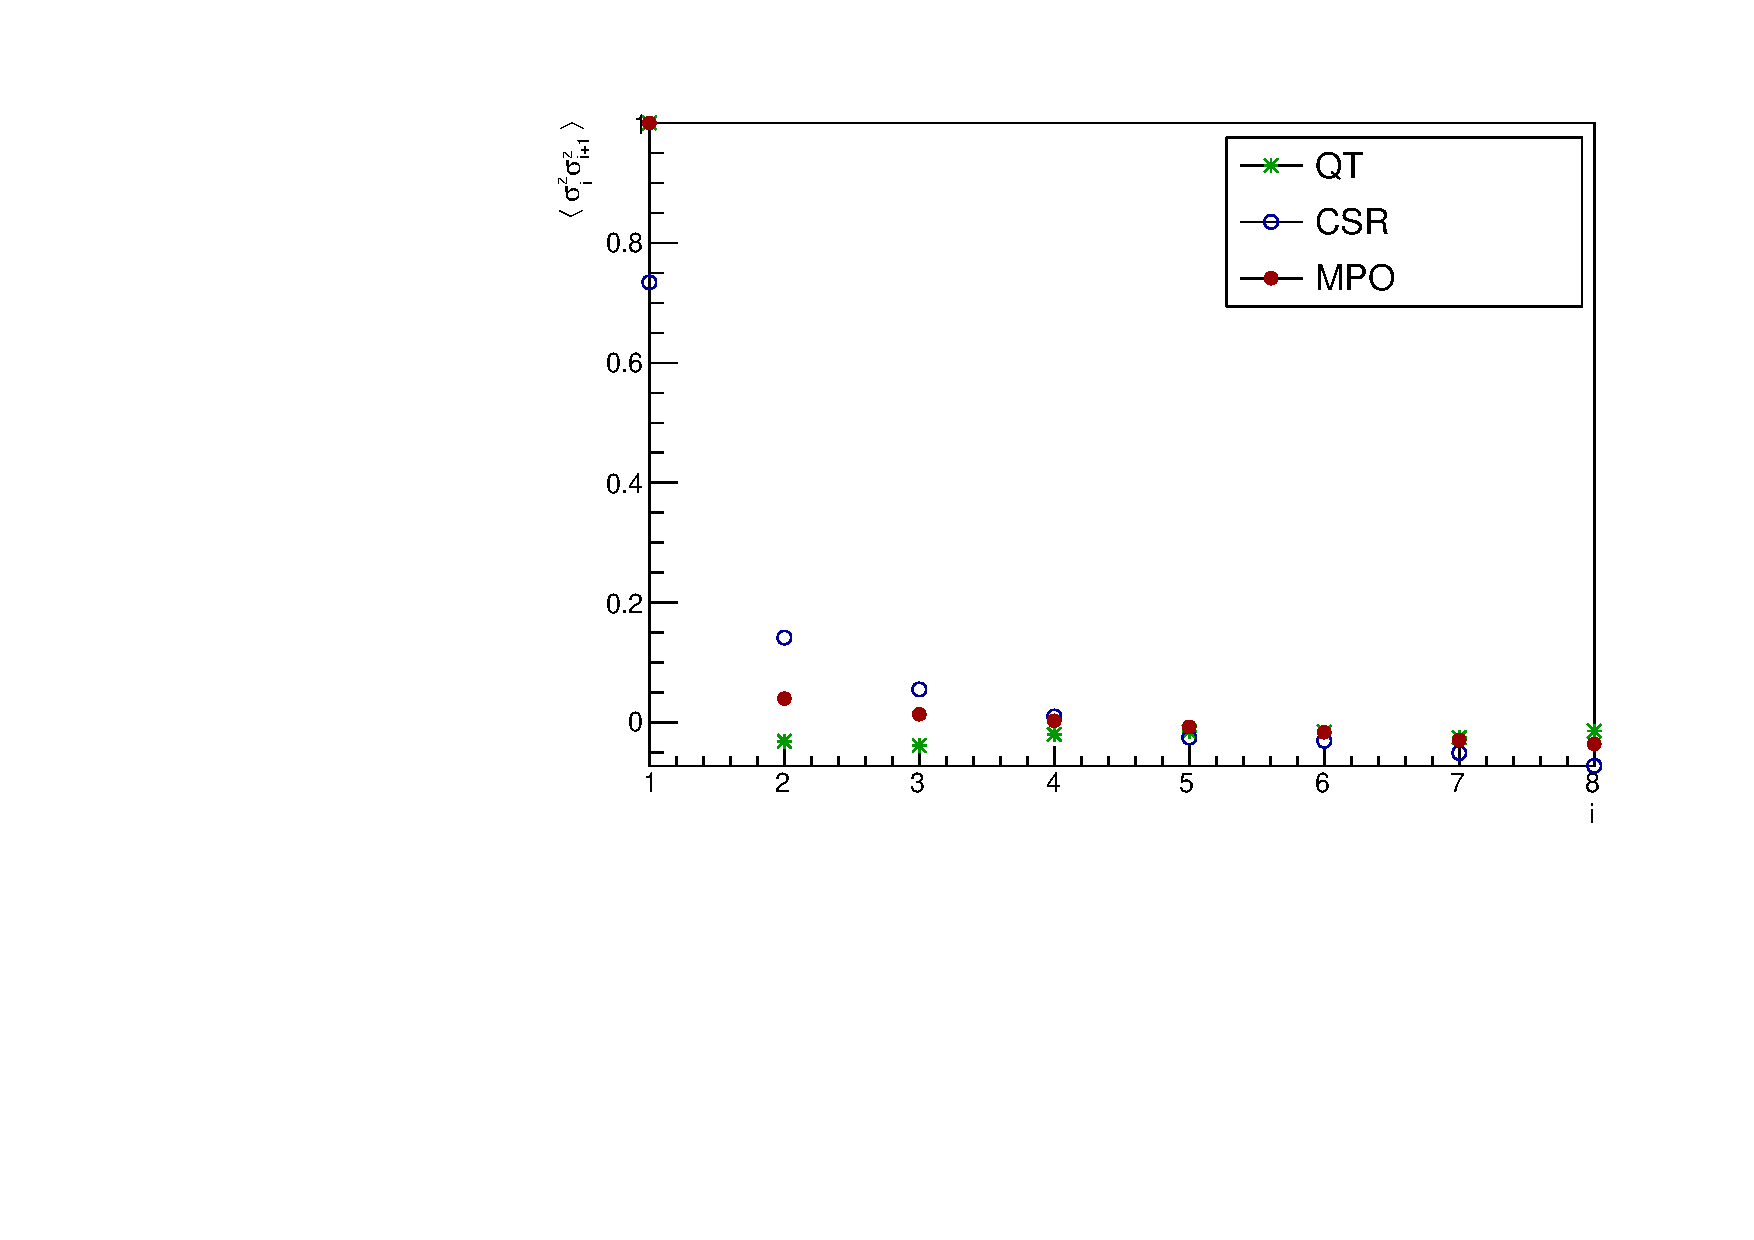
\includegraphics[scale=0.7]{Figures/8sites_comparison/CorrFunc1_8s_J10505.pdf}
    \caption{Correlation function with respect to the spin positioned in the first site of the chain, characterized by $\gamma~=~1, J_x=1, J_y=0.5, J_z=0.5$; \emph{i} stands for the site index.}
    \label{fig:my_label}
\end{figure}

\begin{figure}[H]
    \centering
    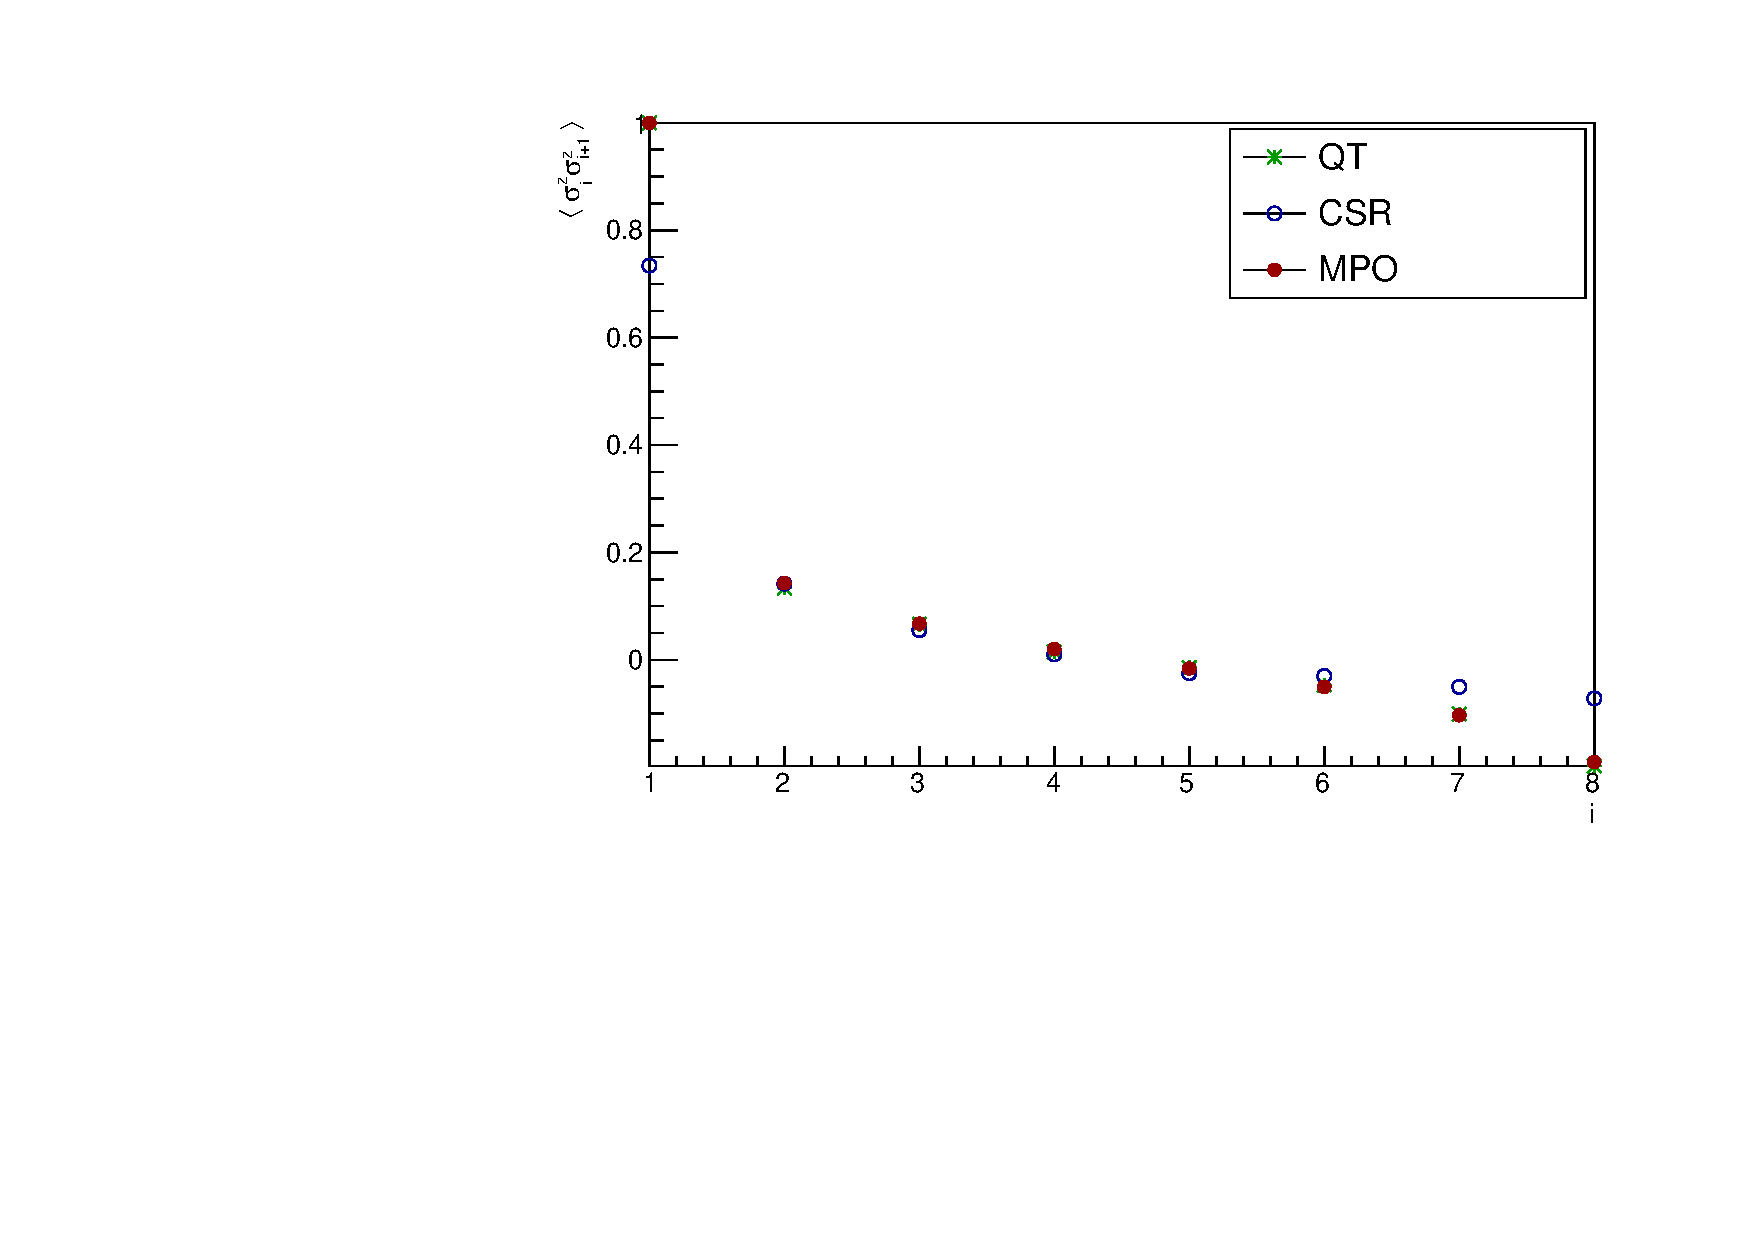
\includegraphics[scale=0.7]{Figures/8sites_comparison/CorrFunc1_8s_J1051.pdf}
    \caption{Correlation function with respect to the spin positioned in the first site of the chain, characterized by $\gamma~=~1, J_x=1, J_y=0.5, J_z=1$; \emph{i} stands for the site index.}
    \label{fig:my_label}
\end{figure}

\begin{figure}[H]
    \centering
    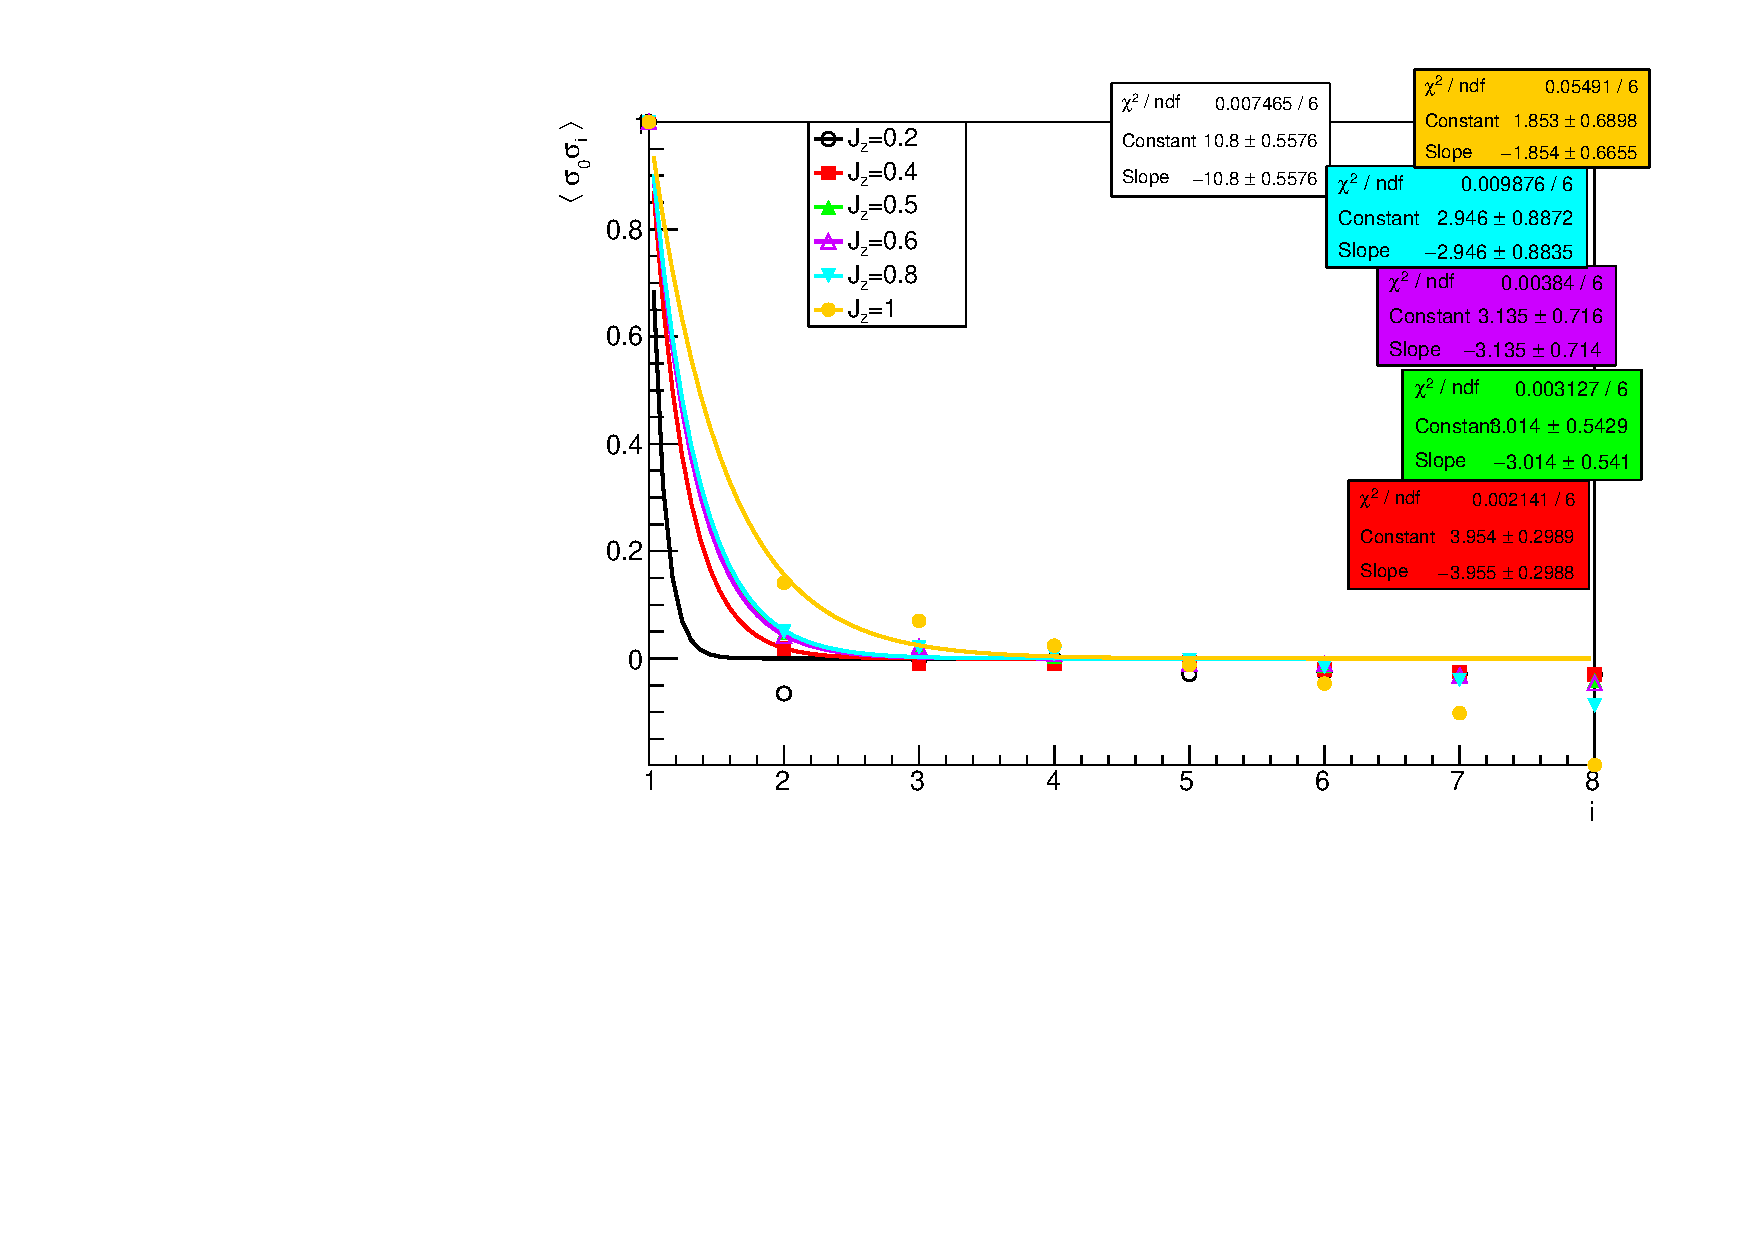
\includegraphics[scale=0.7]{Figures/8sites_comparison/FIT8sCorrFunc1_QT_under1.pdf}
    \caption{Data are obtained from QT method.}
    \label{fig:my_label}
\end{figure}

\begin{figure}[H]
    \centering
    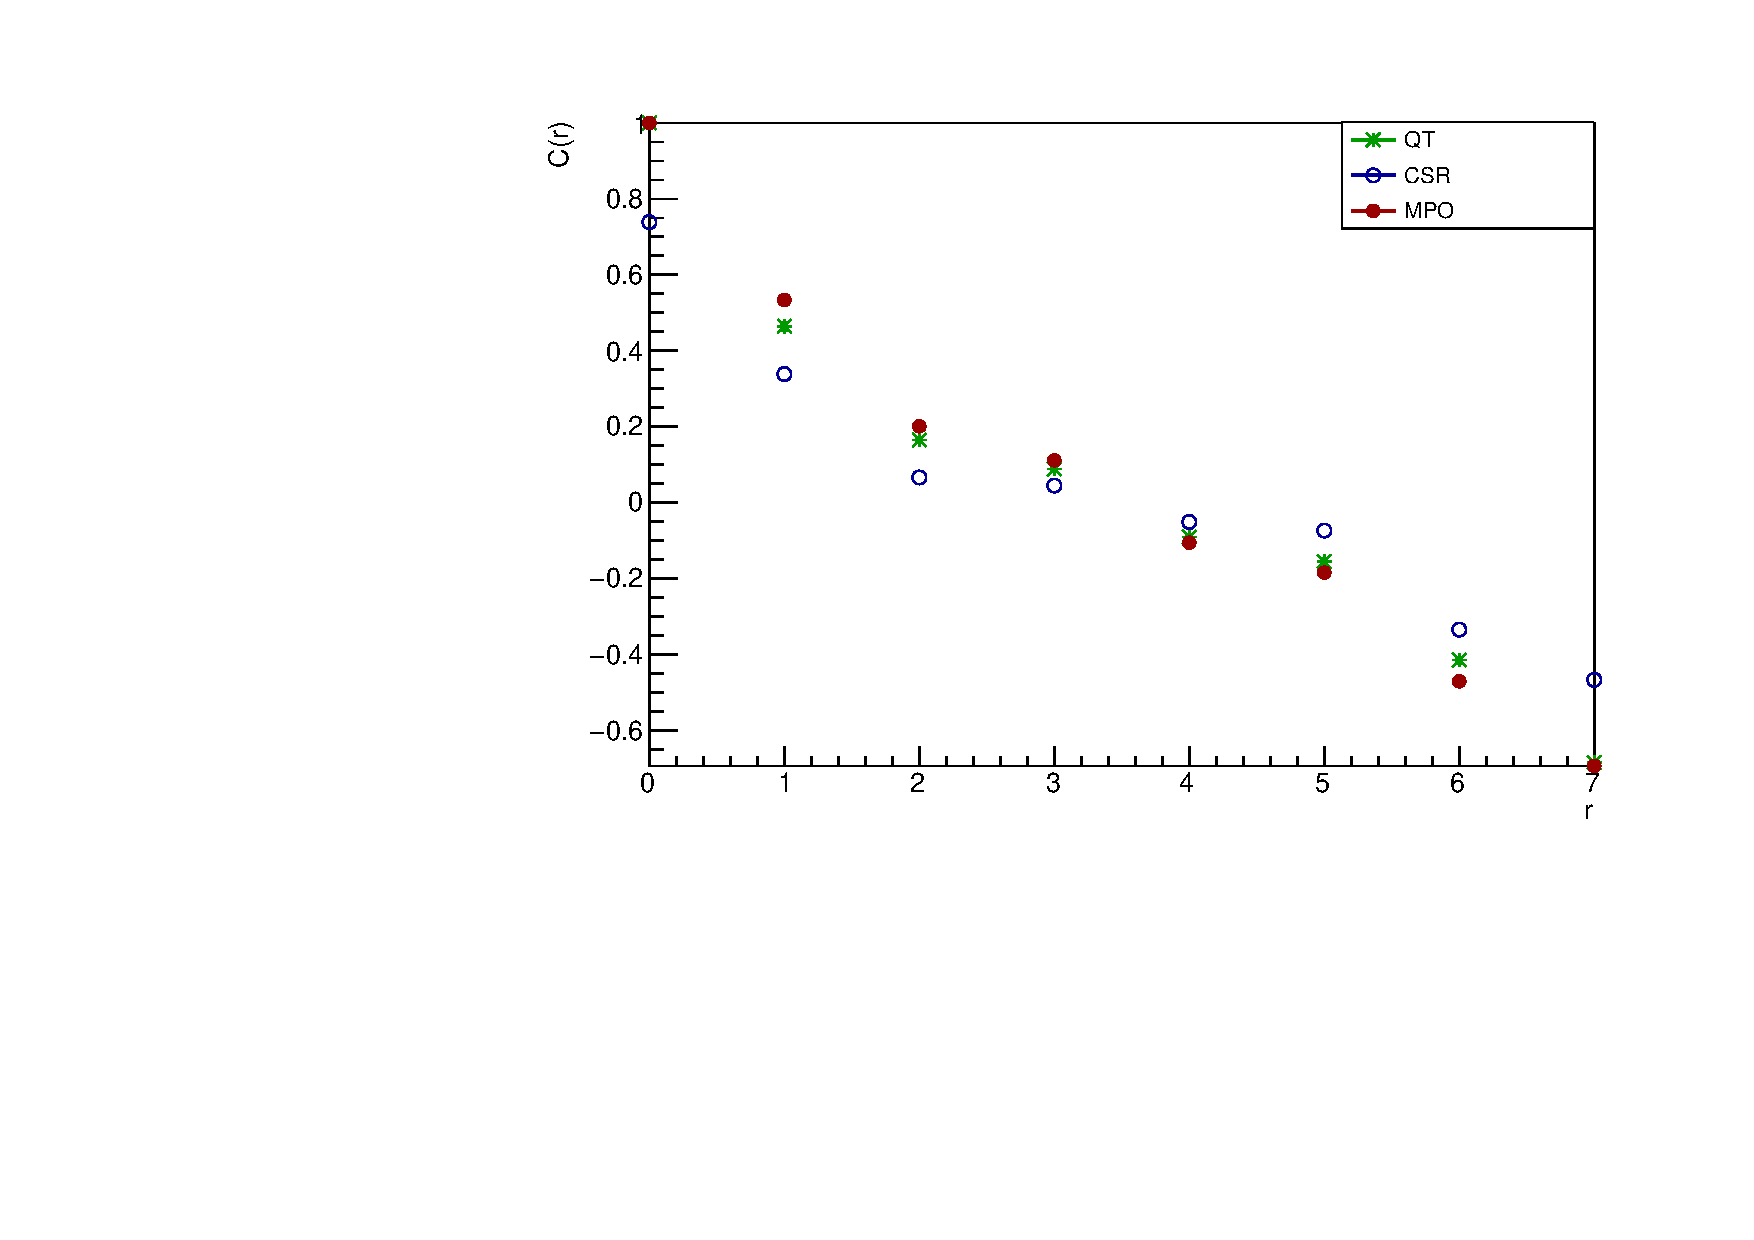
\includegraphics[scale=0.7]{Figures/8sites_comparison/CorrFunc1_8s_J10515.pdf}
    \caption{Correlation function with respect to the spin positioned in the first site of the chain, characterized by $\gamma~=~1, J_x=1, J_y=0.5, J_z=1.5$; \emph{i} stands for the site index.}
    \label{fig:my_label}
\end{figure}

It is interesting how the profile of correlation changes from an exponential behaviour to a linear one. In the following, we will see how this linear profile changes with respect to $\Delta$. The following fits, as all those performed in this thesis, are done by~\cite{root_cern}.

\begin{figure}[H]
    \centering
    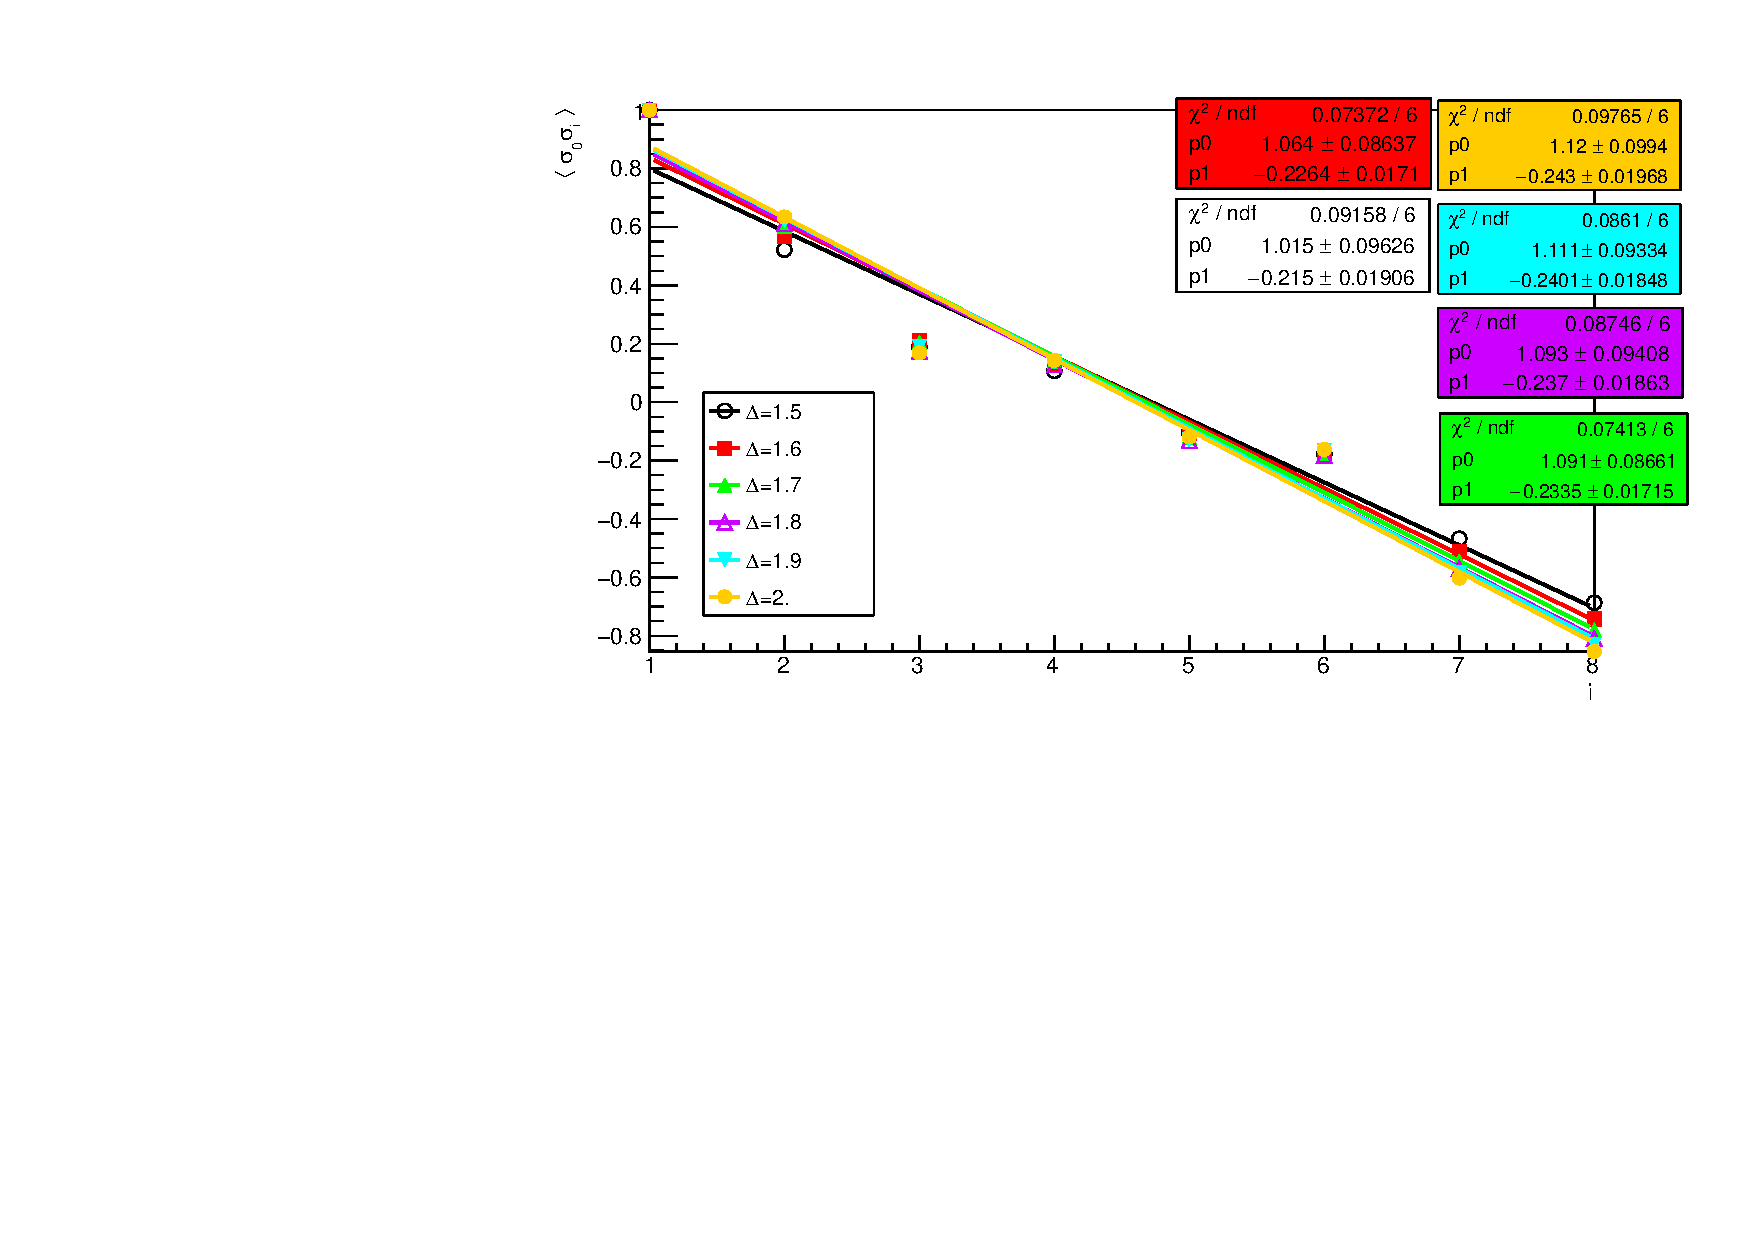
\includegraphics[scale=0.8]{Figures/8sites_comparison/FIT8sCorrFunc1_MPO_over15.pdf}
    \caption{Data are obtained from QT method.}
    \label{fig:my_label}
\end{figure}




\section{Spin Transport}
In this section we are going to study the spin current $j_\sigma$ defined from the continuity equation for the local spin operators~\cite{BenentiCasatiProsenRossini}:
\begin{equation}
    \frac{\partial S^k_z}{\partial t} + \nabla (j_\sigma)_k = 0,
\end{equation}
which can be rewritten as
\begin{equation}
    (j_\sigma)_{k+1}-(j_\sigma)_k = \frac{i}{2}[\sigma_k^z , H],
\end{equation}
where $S_k^z \equiv \sigma_k^z/2$ and where $H$ is the Hamiltonian written in~\ref{ham_chain}. So, we obtain:
\begin{equation}
    j_\sigma = J_y (\sigma_k^x \sigma_{k+1}^y) - J_x (\sigma_k^y \sigma_{k+1}^x).
\end{equation}

\begin{figure}[H]
    \centering
    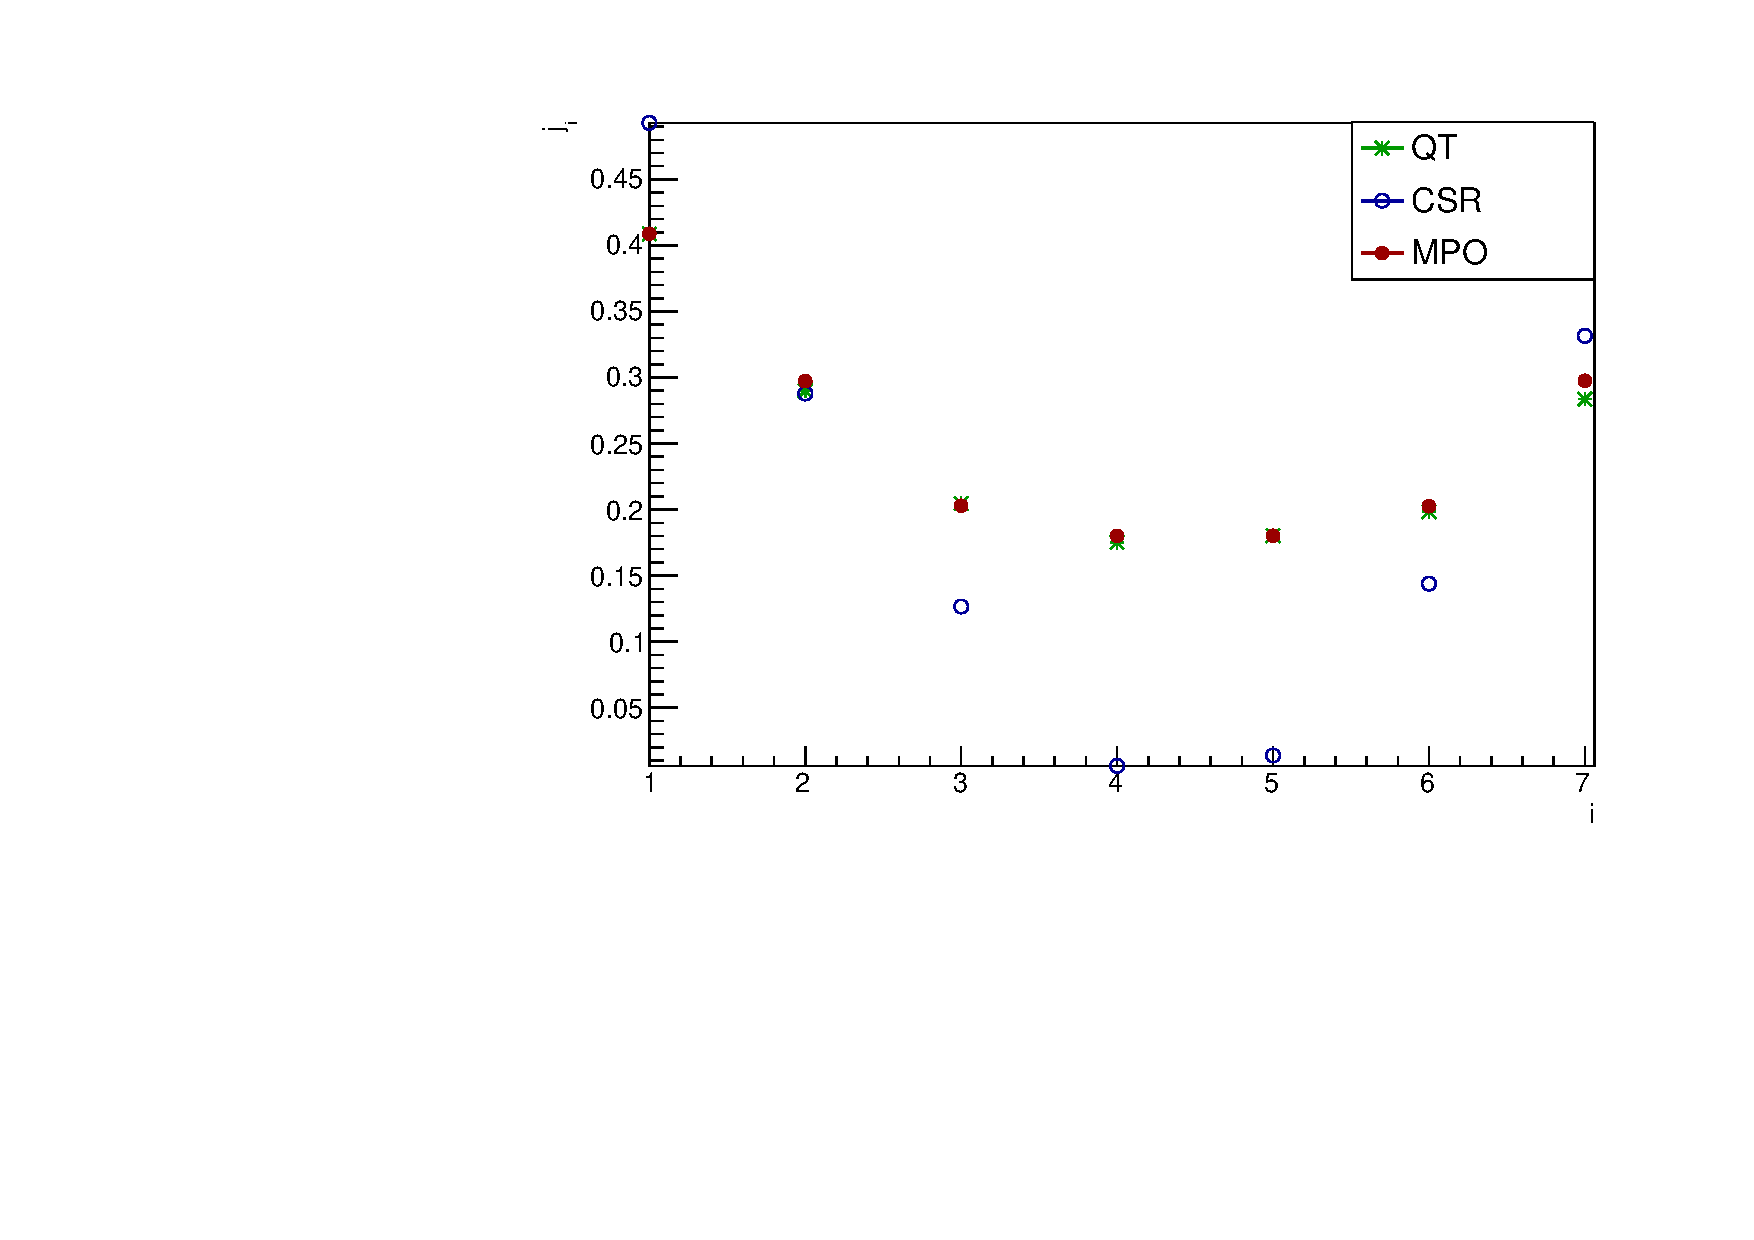
\includegraphics[scale=0.7]{Figures/8sites_comparison/SpinCurr_8s_J10505.pdf}
    \caption{Spin current of the chain, characterized by $\gamma=1, J_x=1, J_y=0.5, J_z=0.5$; \emph{i} stands for the site index.}
    \label{fig:my_label}
\end{figure}

\begin{figure}[H]
    \centering
    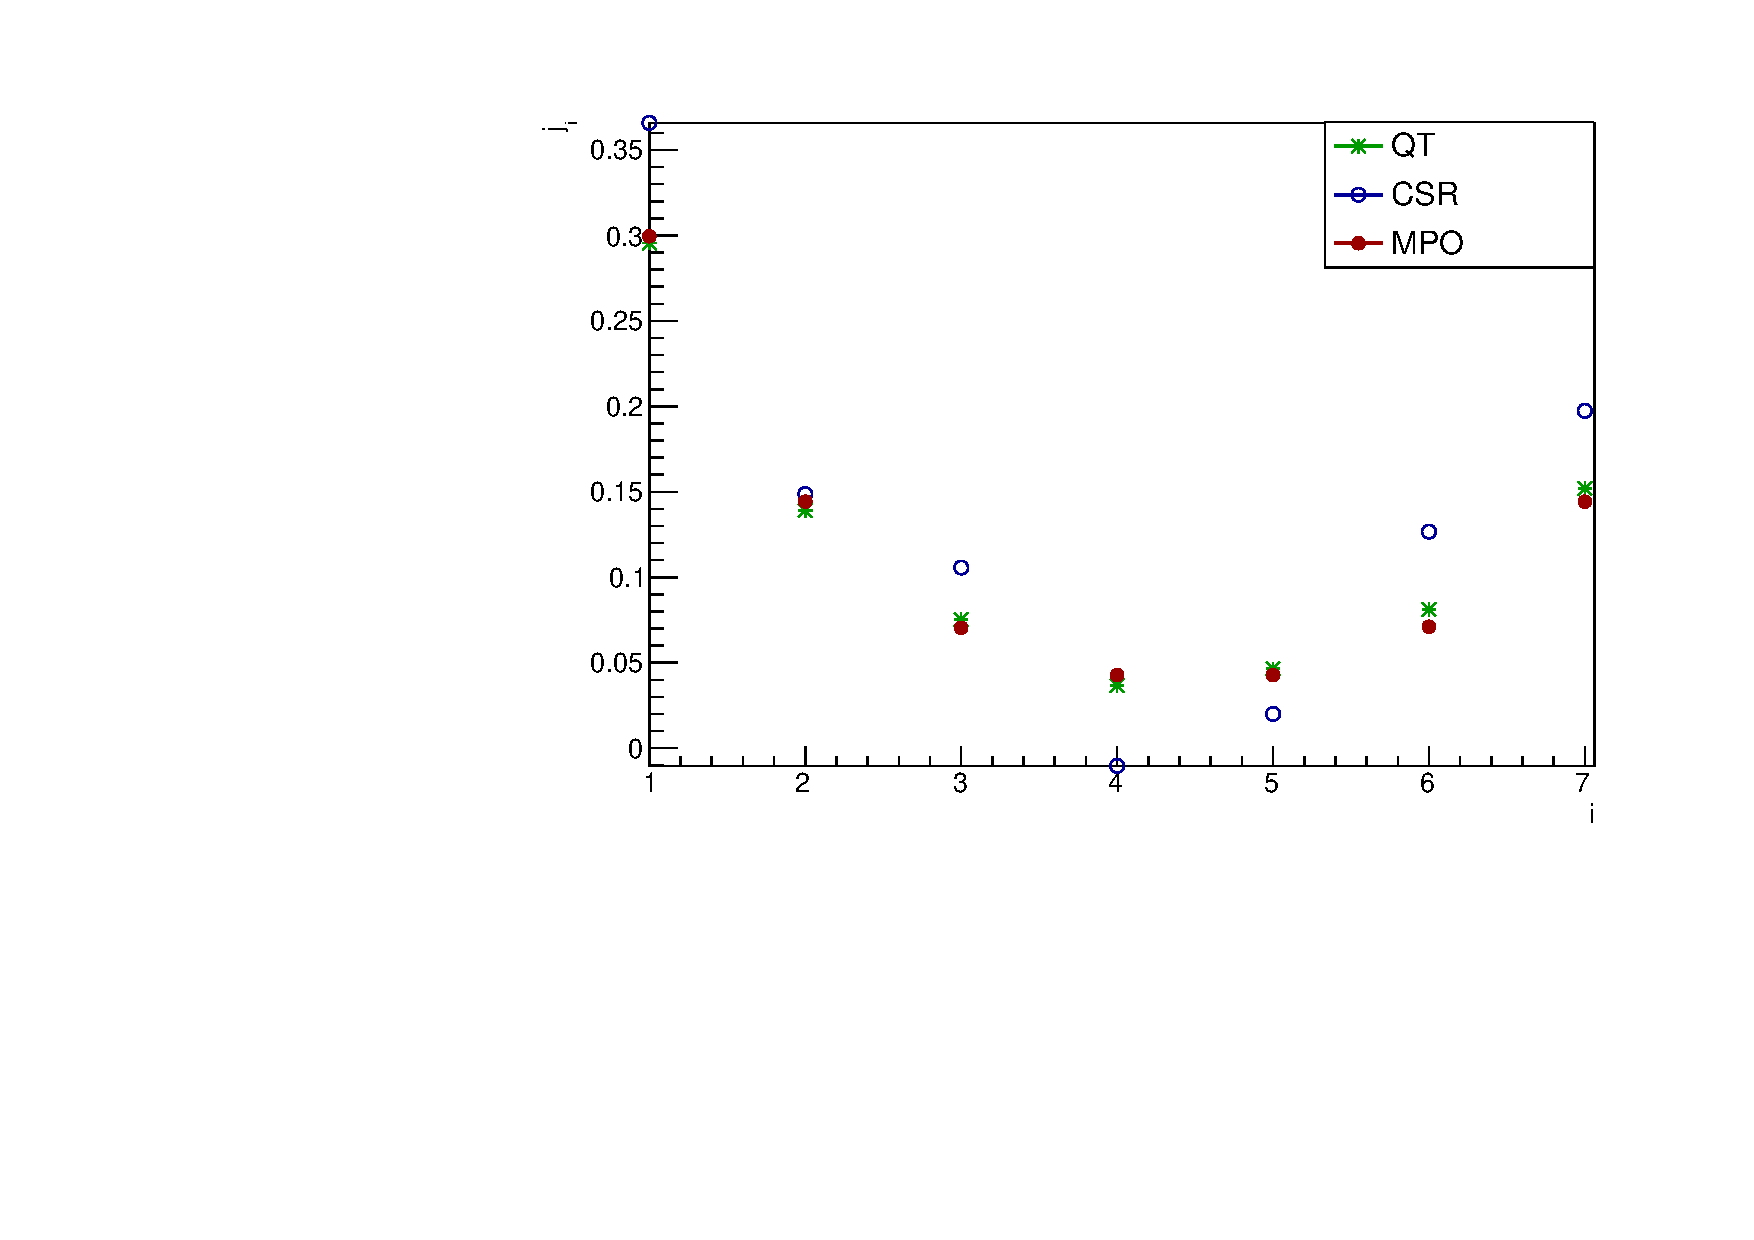
\includegraphics[scale=0.7]{Figures/8sites_comparison/SpinCurr_8s_J1051.pdf}
    \caption{Spin current of the chain, characterized by $\gamma=1, J_x=1, J_y=0.5, J_z=1$; \emph{i} stands for the site index.}
    \label{fig:my_label}
\end{figure}

\begin{figure}[H]
    \centering
    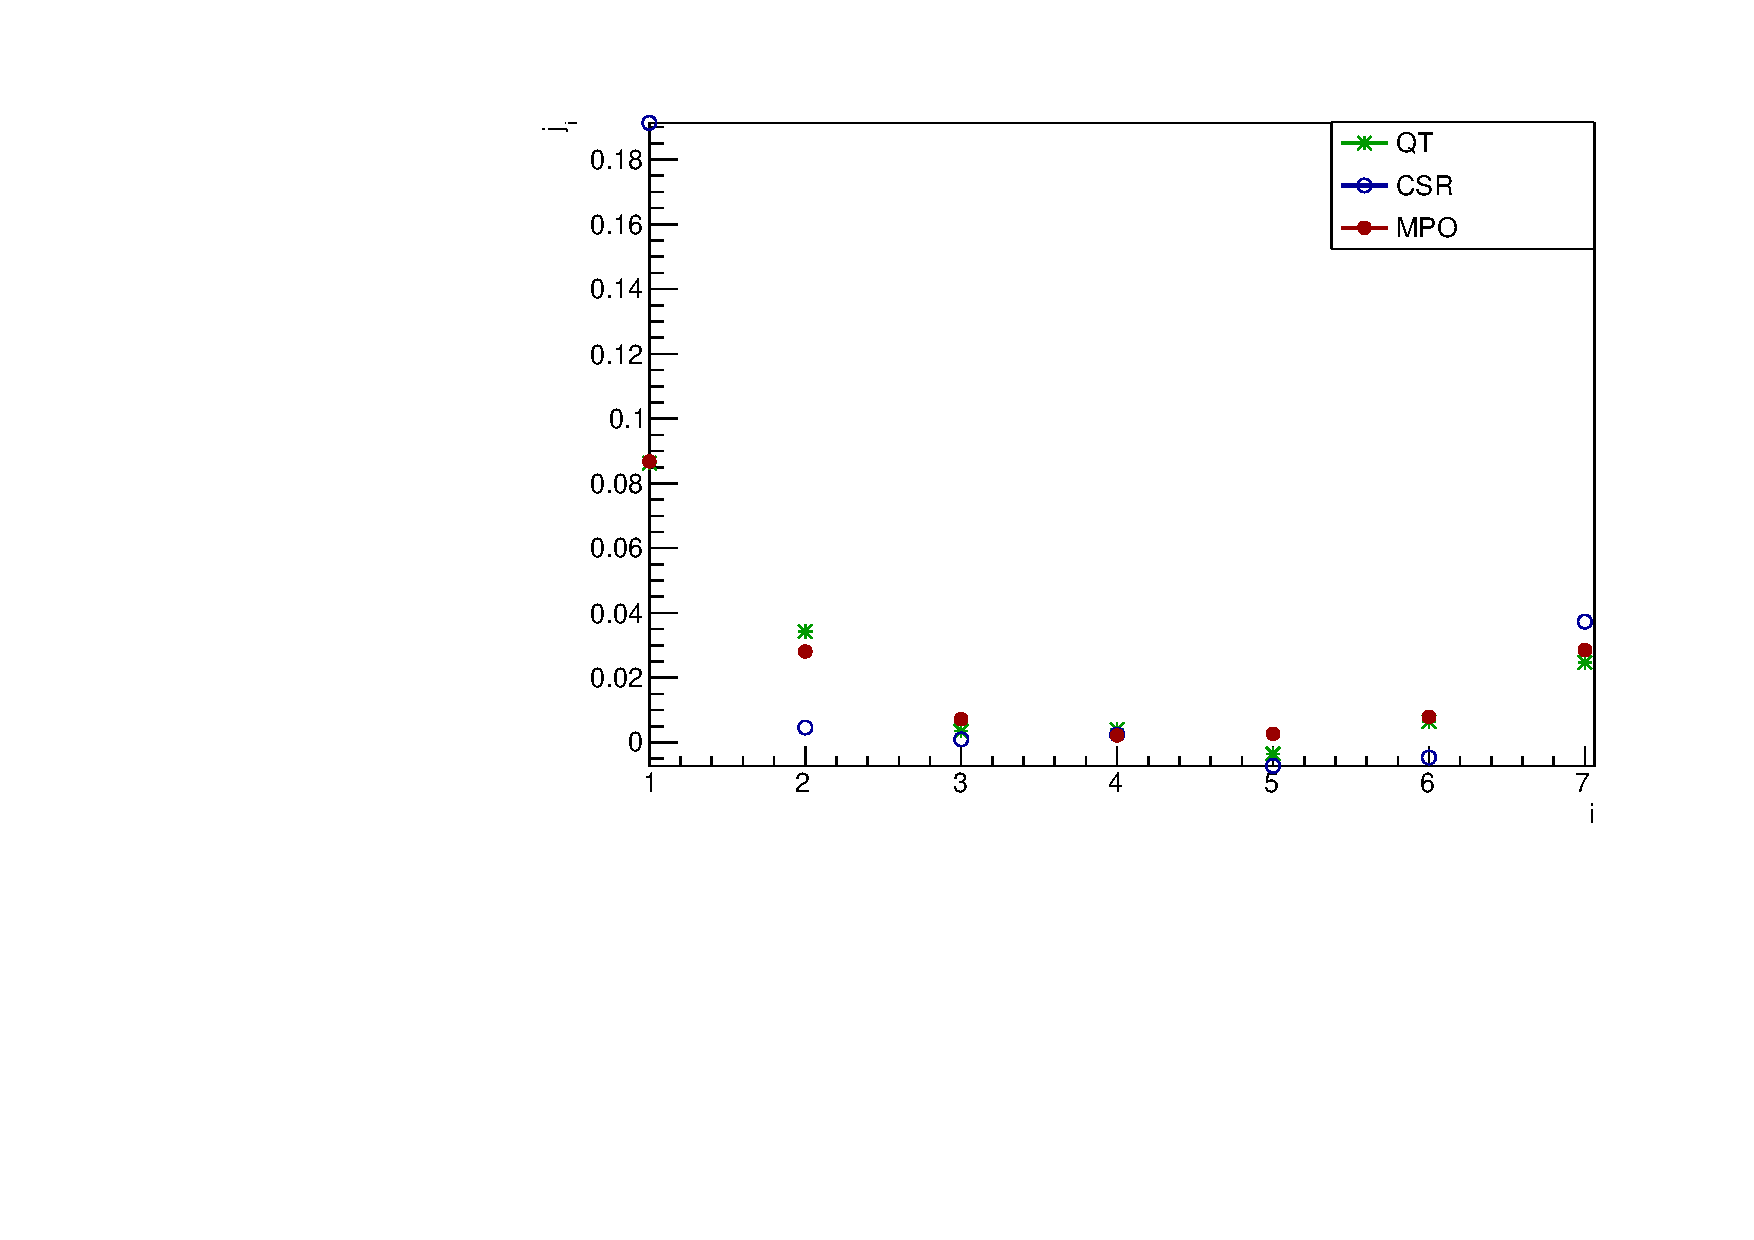
\includegraphics[scale=0.7]{Figures/8sites_comparison/SpinCurr_8s_J10515.pdf}
    \caption{Spin current of the chain, characterized by $\gamma=1, J_x=1, J_y=0.5, J_z=1.5$; \emph{i} stands for the site index.}
    \label{fig:my_label}
\end{figure}

Let us see what happens in the case of a \textbf{12-sites} chain.

\begin{figure}[H]
    \centering
    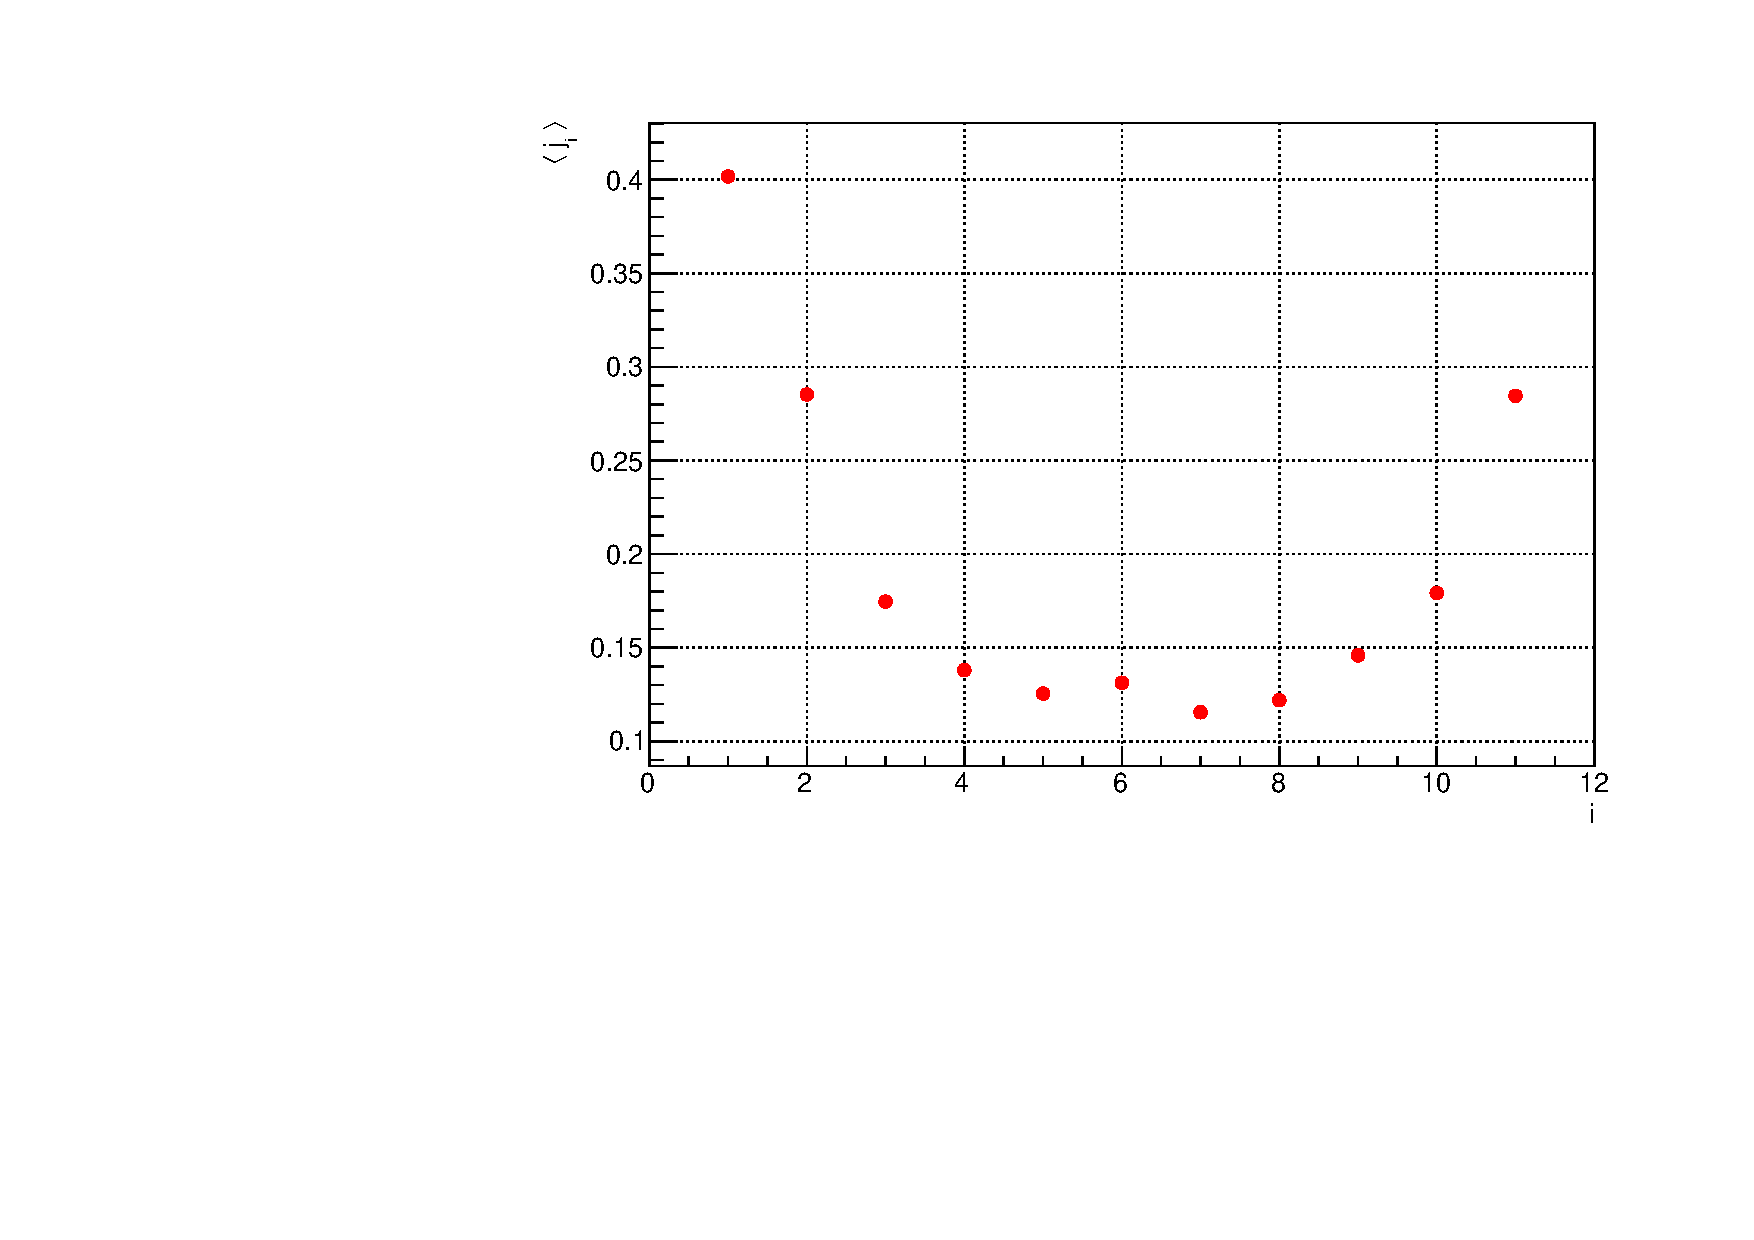
\includegraphics[scale=0.7]{Figures/12sites/SpinCurrL012m060Time002000_J10505.pdf}
    \caption{Spin current of a 12-sites chain, characterized by $\gamma=1, J_x=1, J_y=0.5, J_z=0.5$; \emph{i} stands for the site index. Data are obtained from MPO method.}
    \label{fig:my_label}
\end{figure}

\begin{figure}[H]
    \centering
    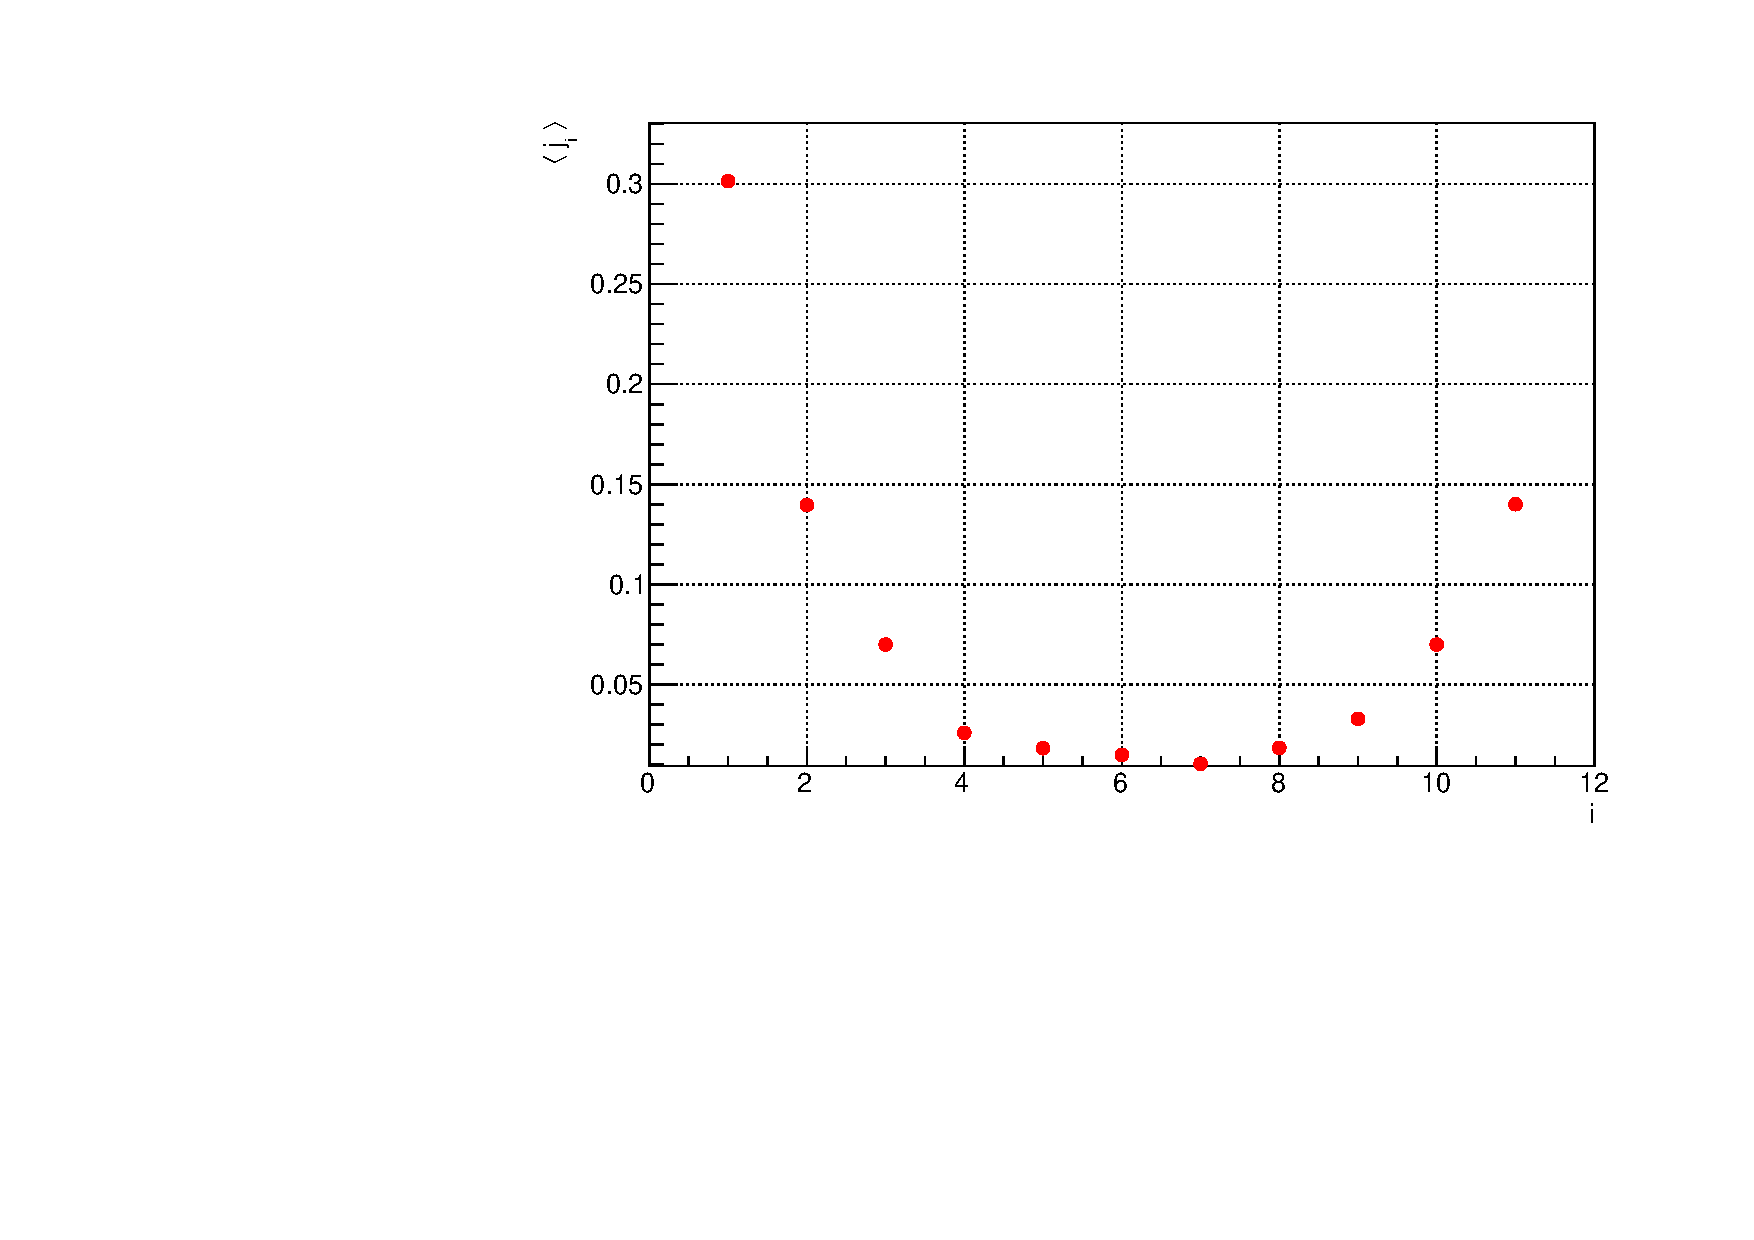
\includegraphics[scale=0.7]{Figures/12sites/SpinCurrL012m060Time002000_J1051.pdf}
    \caption{Spin current of a 12-sites chain, characterized by $\gamma=1, J_x=1, J_y=0.5, J_z=1.$; \emph{i} stands for the site index. Data are obtained from MPO method.}
    \label{fig:my_label}
\end{figure}

\begin{figure}[H]
    \centering
    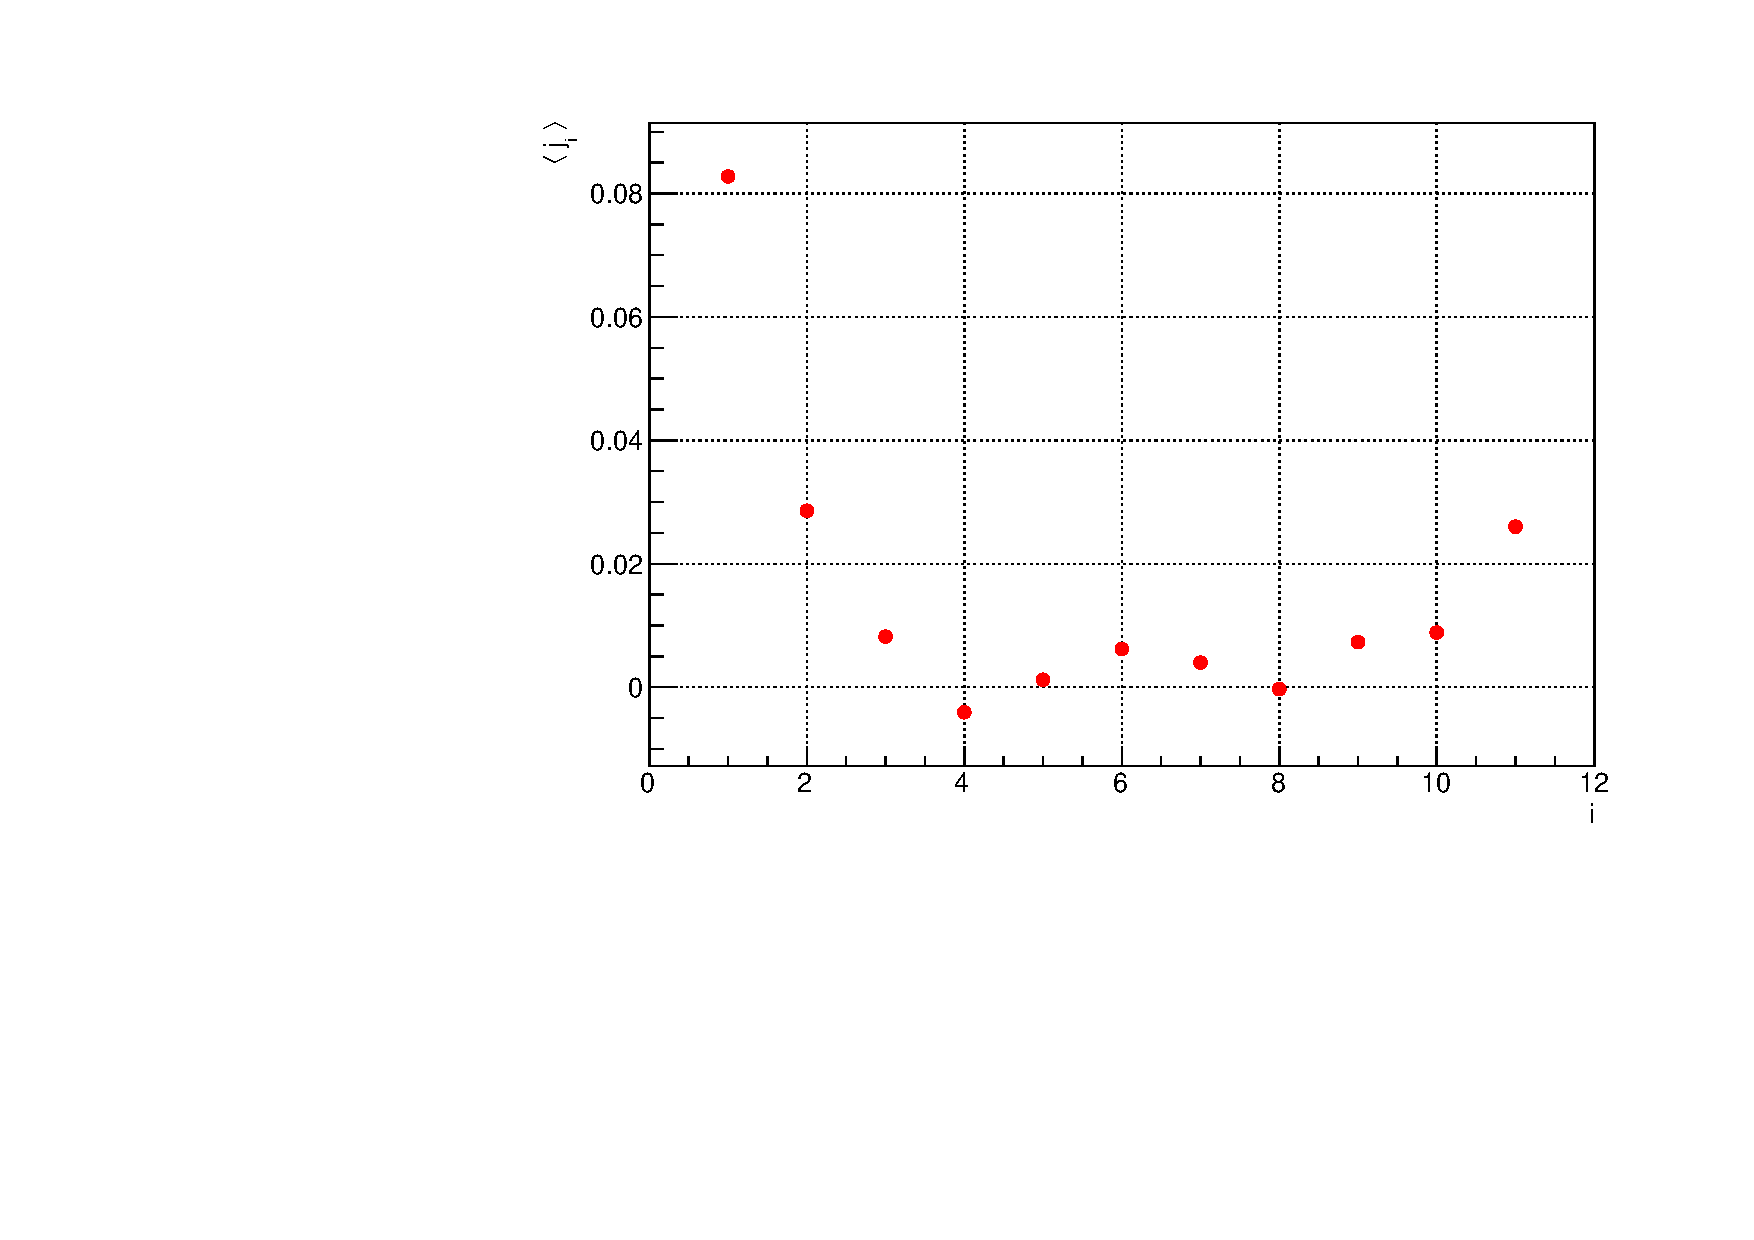
\includegraphics[scale=0.7]{Figures/12sites/SpinCurrL012m060Time002000_J10515.pdf}
    \caption{Spin current of a 12-sites chain, characterized by $\gamma=1, J_x=1, J_y=0.5, J_z=1.5$; \emph{i} stands for the site index. Data are obtained from MPO method.}
    \label{fig:my_label}
\end{figure}